\documentclass[conference]{IEEEtran}
\IEEEoverridecommandlockouts
% The preceding line is only needed to identify funding in the first footnote. If that is unneeded, please comment it out.
\usepackage{cite}
\usepackage{amsmath,amssymb,amsfonts}
\usepackage{algorithmic}
\usepackage{graphicx}
\usepackage{textcomp}
\usepackage{xcolor}
\usepackage{graphicx}
\usepackage{lipsum}
\usepackage[pangram]{blindtext}
\usepackage{soul}
\sethlcolor{black}

\ifCLASSOPTIONcompsoc
    \usepackage[caption=false, font=normalsize, labelfont=sf, textfont=sf]{subfig}
\else
\usepackage[caption=false, font=footnotesize]{subfig}
\fi
\def\BibTeX{{\rm B\kern-.05em{\sc i\kern-.025em b}\kern-.08em
    T\kern-.1667em\lower.7ex\hbox{E}\kern-.125emX}}

\makeatletter 
\newif\if@blind
\@blindtrue %use \@blindfalse on final version
\if@blind \sethlcolor{black}\else
   \let\hl\relax
\fi
\def\BibTeX{{\rm B\kern-.05em{\sc i\kern-.025em b}\kern-.08em
    T\kern-.1667em\lower.7ex\hbox{E}\kern-.125emX}}
    
\newcommand{\linebreakand}{
	\end{@IEEEauthorhalign}
	\hfill\mbox{}\par
	\mbox{}\hfill\begin{@IEEEauthorhalign}
}
\makeatother
% % Vector
% \newcommand{\vect}[1]{\vec{#1}}
% \renewcommand{\vec}[1]{\bm{#1}}
% % Matrix
% \newcommand{\mat}[1]{\bm{\mathrm{#1}}}

\begin{document}

\title{Towards Predictive Maintenance: an Edge Data-based Vibration Monitoring System in Industry 4.0}

\author{\IEEEauthorblockN{\hl{Victor L. L. Costa and Bj{\"o}rn Eberhardt}}
\IEEEauthorblockA{\textit{} 
\textit{\hl{Delta Systems GbR}}\\
\hl{Aachen, Germany} \\
\hl{\{costa, eberhardt\}@delta-systems.de}}

\and
\IEEEauthorblockN{\hl{Jiahang Chen and J{\"u}rgen Ro{\ss}mann}}
\IEEEauthorblockA{\textit{} 
\textit{\hl{Institute for Man-Machine Interaction}}\\
\textit{\hl{RWTH Aachen University}}\\
\hl{Aachen, Germany} \\
\hl{\{chen, rossmann\}@mmi.rwth-aachen.de}
}

%\linebreakand
%\IEEEauthorblockN{Bj{\"o}rn Eberhardt}
%\IEEEauthorblockA{\textit{Delta Systems GbR} \\
%Aachen, Germany \\
%eberhardt@delta-systems.de
%}

%\and
%\IEEEauthorblockN{J{\"u}rgen Ro{\ss}mann}
%\IEEEauthorblockA{\textit{Institute for Man-Machine Interaction} \\
%\textit{RWTH Aachen University}\\
%Aachen, Germany \\
%rossmann@mmi.rwth-aachen.de}
%
}

\maketitle

\begin{abstract}
Due to the high acquisition and operation cost of industrial machinery, the cost-effectiveness is highly affected by the quality and continuity of their production. In this context, Predictive Maintenance emerges as a maintenance strategy aiming to maximize uptime by constantly monitoring a quantity related to the machine's health, such as vibration patterns, in order to perform maintenance stops only when strictly required. The implementation of this strategy, however, faces multiple challenges. One of them is related to the design, installation, and operation of the required sensory systems, which are subjected to budget constraints and technical constraints such as sensor battery lifetime. Another challenge is given by the intelligence required for analyzing real-world data generated within uncontrolled industrial environments and producing a machinery health indicator from it. This paper illustrates a vibration monitoring system currently operating in a textile manufacturing machine; proposes a versatile Anomaly-Detection-based procedure towards analyzing unlabeled real-world data produced by such systems and extracting a machine health indicator from it, while considering energy consumption; and also proposes an extension to the system in order to adapt it to the connectivity requirements set by the current context of Industry 4.0.
\end{abstract}

\begin{IEEEkeywords}
Predictive Maintenance, Anomaly Detection, Vibration Monitoring
\end{IEEEkeywords}

\section{Introduction}

\subsection{The Way to Predictive Maintenance}

Today’s industrial machinery (e.g. textile machine; see Fig. \ref{fig_machine}) are usually capital-intensive. Hence, keeping such equipment in optimal operating condition with the highest availability, performance, and quality is viewed as a crucial part of ensuring the return on investment in the acquisition and operation. In this context, machine maintenance ensures the Overall Equipment Effectiveness (OEE) by satisfying production schedules, minimizing machinery downtime, and preventing potential accidents in workplaces (\cite{chong2015}, \cite{b1}). 

\begin{figure}[htbp]
\centering
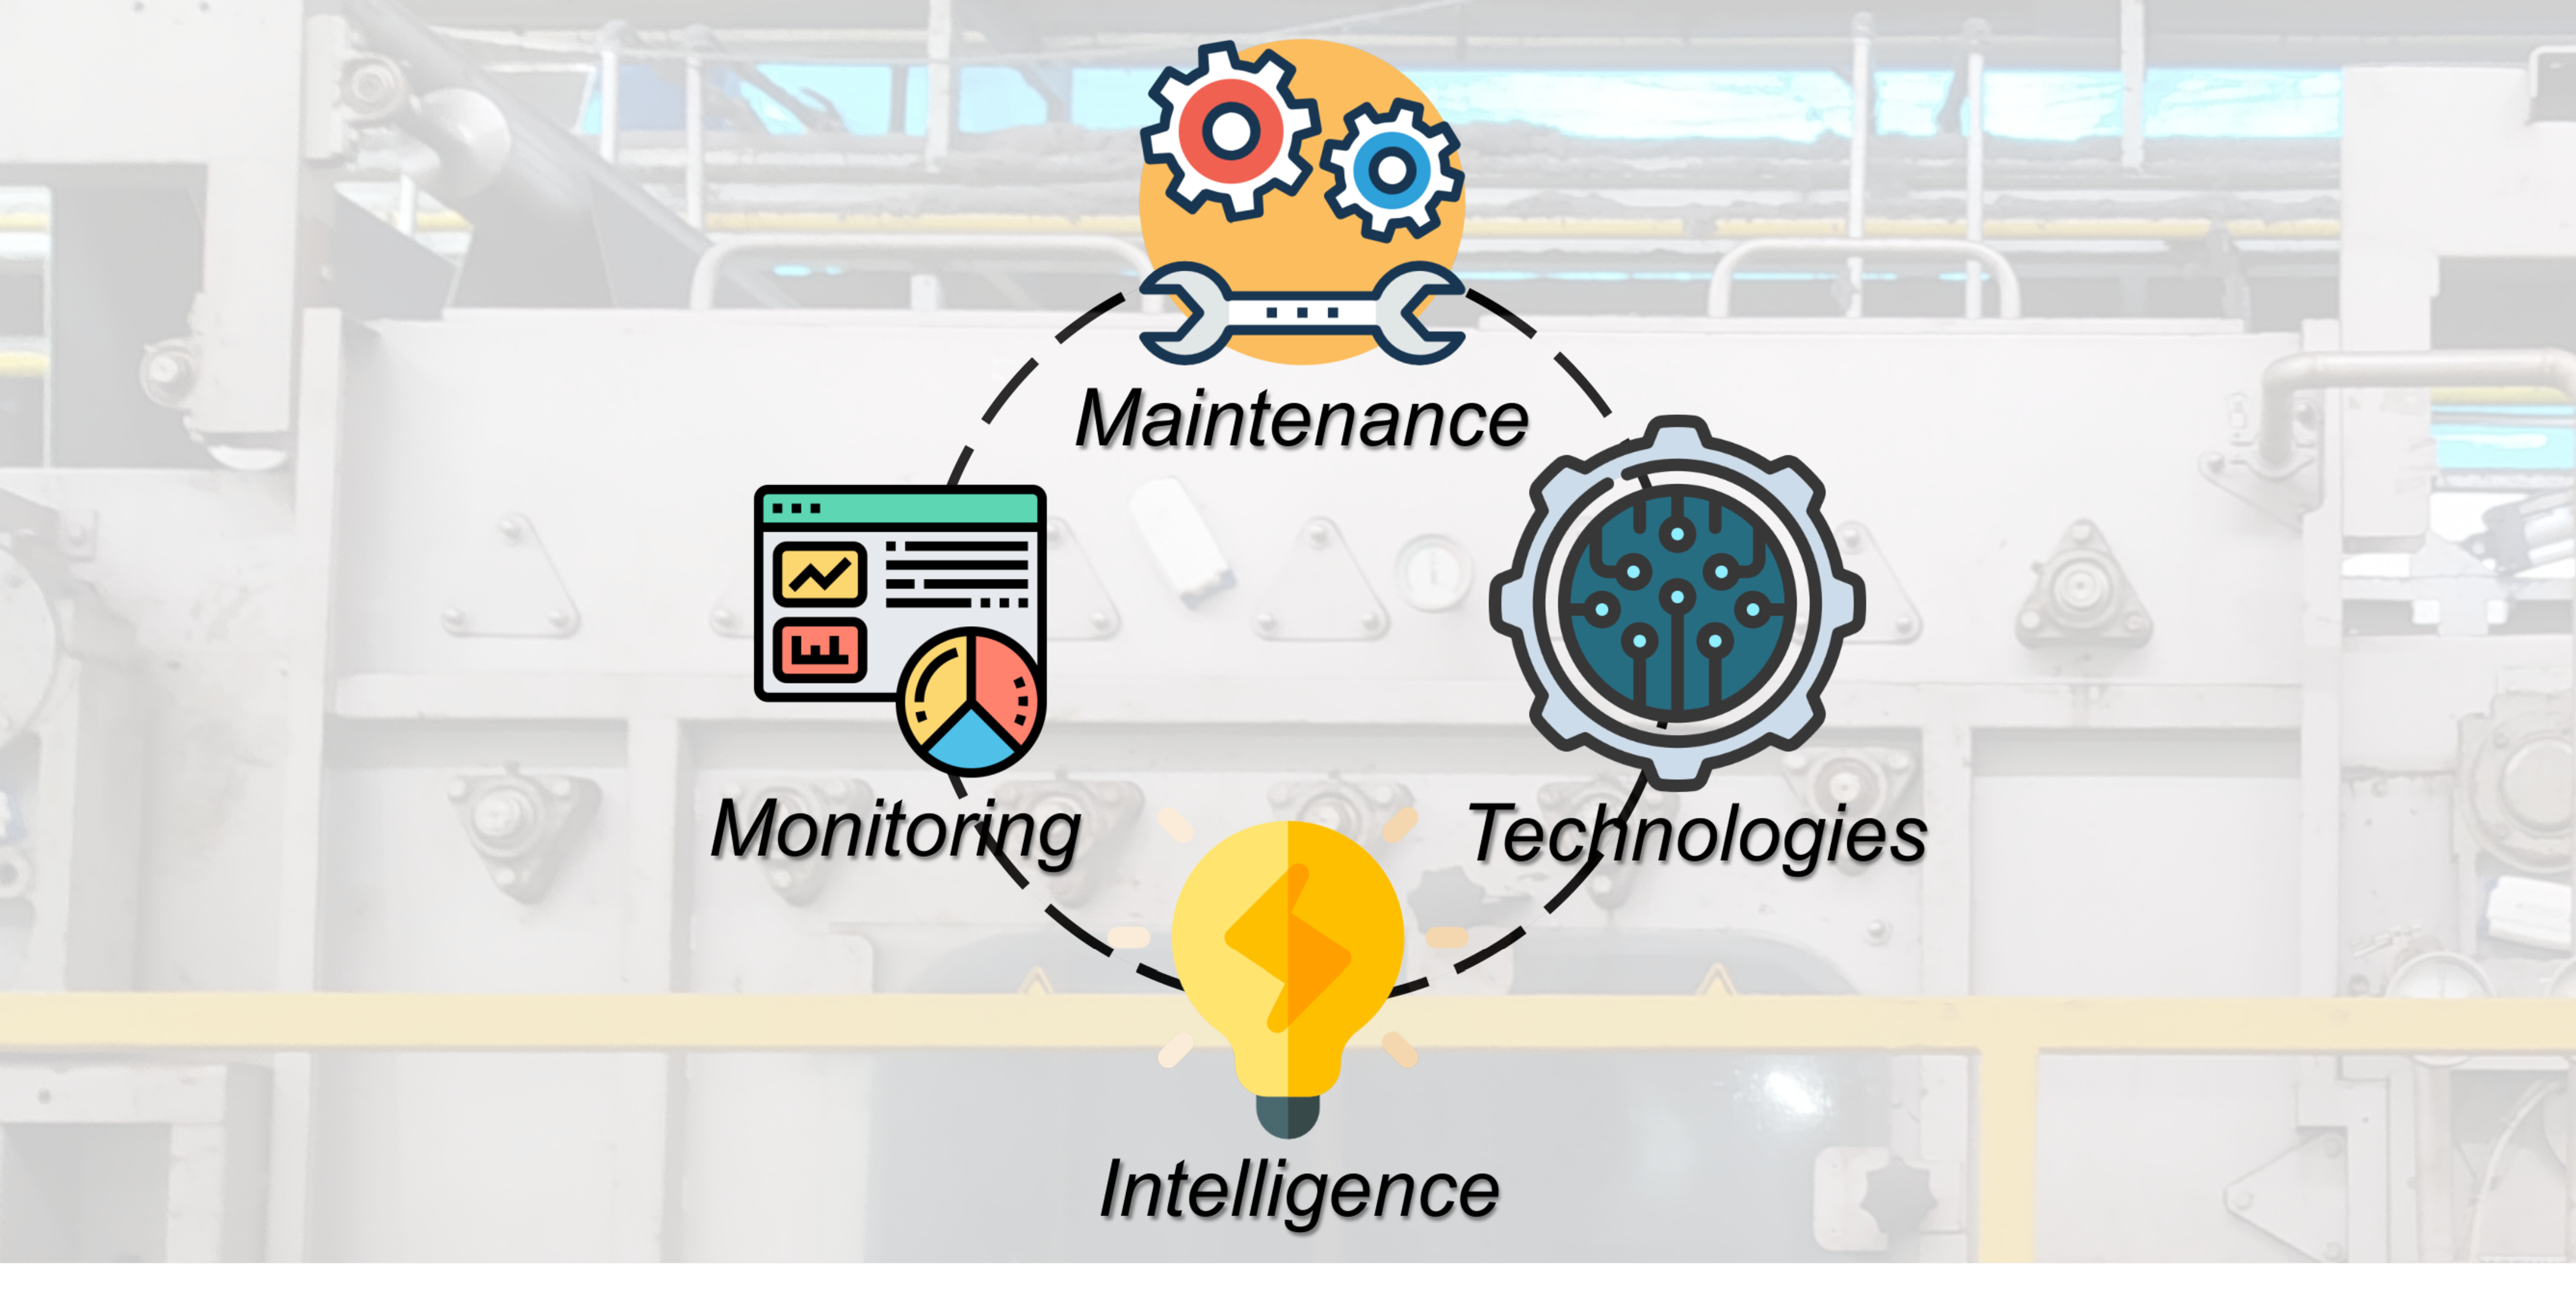
\includegraphics[width=0.4\textwidth]{graphics/predictive_maintenance.pdf}
\caption{Predictive maintenance is a federation of different technologies to monitor the condition of in-service equipment and estimate maintenance stops, delivering machinery with intelligence (textile machinery source: DELTA systems GbR)}
\label{fig_machine}
\end{figure}

Different maintenance strategies are proposed as the complexity of machinery and their working environment increase over time. In general, they can be divided into \cite{b1}:

\begin{itemize}
	\item Reactive Maintenance: performing maintenance when the machine fails
	\item Preventive Maintenance: performing maintenance regularly (every day, week, month ...)
	\item Predictive Maintenance: performing maintenance only shortly before the machine reaches breaking determined by a prediction service
\end{itemize}

Compared to reactive and preventive maintenance, predictive maintenance prevents unnecessary maintenance stops and unscheduled machine downtime.

\subsection{Associated Challenges}
\label{sec_associated_challenges}

Developing predictive maintenance concepts is encountered a wide range of challenges, such as cost, operational variability, and data privacy. 1) as predictive maintenance is based on machine's monitoring data collected from different sensors, the cost of the acquisition and installation of sensors can vary according to the complexity of the data model applied. 2) Individual machines of a same manufacturer model might operate differently under different conditions. Hence, ensuring the general availability of the data-based model leads to issues when the machines operate in different conditions. 3) Accompanied by the increased complexity of methods and the quality of data flow, the hardware requirements for the sensors become stricter. 4) Data always implicates some sensitive information about production and business. Preventing data tampering and leakage must be considered as well.

\subsection{Industry 4.0 - Enabling Predictive Maintenance}

In the current context of Industry 4.0, large amounts of devices are internetworked. The term Internet of Things (IoT) emerges as the amalgamation of software techniques, communication technologies, and individual devices that constitute these networks which may or may not be connected to the internet despite the name.

The emerging chip technology facilitates the development of edge devices which in comparison to cloud devices, provide the following advantages: 1) reduced latency, 2) improved security, 3) reduced infrastructure cost, 4) improved reliability, and 5) large autonomy for battery-powered devices. The combination of edge devices and predictive maintenance covers the challenges mentioned above.

\subsection{Our Contribution}

This paper illustrates an edge-based vibration monitoring system currently operating in a textile manufacturing machine. It proposes a versatile anomaly-detection-based procedure for the analysis of real-world data and extraction of machine health status, considering the battery life of sensors.

The remaining part of the paper is structured as follows: Section \ref{sec_related_work} provides an overview of work related to predictive maintenance concepts for vibration analysis. In Section \ref{sec_concept}, we propose our concept for data analysis techniques. The implementation details are presented in Section \ref{sec_implementation}. We highlight the results of the data analysis and indicate our discussion in Section \ref{sec_results_discussion}. Consequently, the paper is concluded in Section \ref{sec_conclusion}.



\section{Related Work}
\label{sec_related_work}

In the context of predictive maintenance, there is a wide range of successful applications across diverse industries, for example, \cite{adebiyi}, \cite{alnajjar}, and \cite{doyleek}. Nevertheless, the failure rate of implementing predictive maintenance remains at a certain high level since it is complicated to balance the requirements of various conflicting priorities, such as a dynamically changing environment, inaccurate plant model, and high energy consumption in battery-constrained devices. An exploration of the challenges and strategies involved in achieving success in implementing predictive maintenance is found in \cite{carnero2006evaluation}.

In the area of rotating machinery, people always seek practical approaches to enhance system uptime of operation. One solution refers to the utilization of predictive maintenance, in which vibration analysis presents a significant potential, as denoted in \cite{b1}. This also discusses in detail the fundamentals required for the development of physics-based solutions.

In addition, data-based approaches, which shift the focus of the intelligence required from expert knowledge to historical data, are implemented in numerous studies. For example, \cite{wu2017remaining} and \cite{li2020lifelong} present vibration-based PM methods with labeled data obtained from experiments in controlled conditions. Another approach is given in \cite{cui2018anomaly}, which presents a condition monitoring approach for wind power equipment in field operating conditions. The respective modeling also uses labeled data and a type of machine which works with low operational variability.

Overall, the authors in \cite{wu2017remaining} and \cite{li2020lifelong} use data collected from experiments within ideal conditions, e.g., the machine was working without disturbances caused by temperature variations, human operation interference, cross-effects from other parts of the industry, and so on. Hence, the experimental setup can ensure that no external effects affect the data being produced. 

In our work, data is collected from a machine that operates in a real-world scenario. Hence, external effects mentioned above must be considered, e.g., a machine produces typically quite different data in summer and winter respectively, although it performs the same task. Our work, unlike other approaches available in various other literature, aims to detect different operational modes with unlabeled data, despite variable conditions and external effects.

% ===============================================================
% ===============================================================
% ===============================================================
\section{Concept - Data Analysis Techniques}
\label{sec_concept}

The vibration monitoring solution proposed in this work employs various data and signal analysis techniques. This section is dedicated to summarizing them; see Fig. \ref{techniques_overview}. 

%First, in Section \ref{sec_vibration_analysis}, we present a discussion about the field of machine vibration analysis, which is required in order to gain insights into how to interpret the vibration signals and learn which of its features can be correlated to the machine's condition. In Section \ref{sec_signal_processing} we present an overview of the implemented signal processing techniques to extract the desired features from the vibration signals. In Section \ref{sec_clustering} we discuss the data clustering techniques used to identify and segregate the potentialy multiple operational modes presented by the machine under study. Finaly, in Section \ref{sec_anomaly_detection} we explore the Anomaly Detection concept and discuss about how to use the multi-variate Gaussian distribution to implement Anomaly Detection in the scenario at hand.

\begin{figure}[htbp]
\centerline{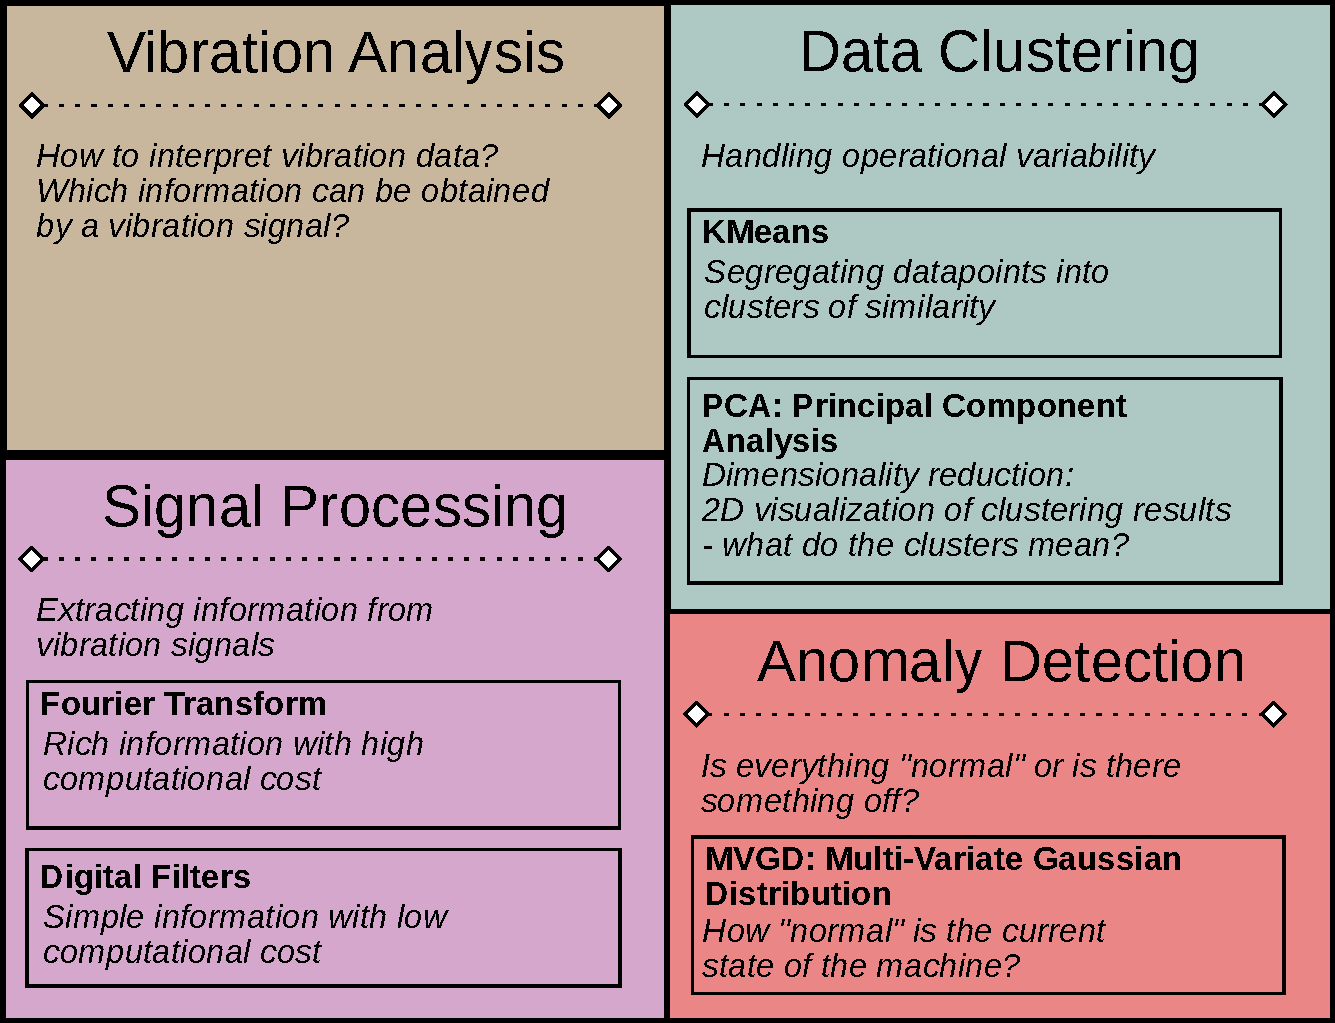
\includegraphics[width=\columnwidth]{graphics/techniques/techniques_block.pdf}}
\caption{A brief overview of the techniques employed in the data analysis}
\label{techniques_overview}
\end{figure}



% ===============================================================
\subsection{Vibration Analysis}
\label{sec_vibration_analysis}
% RMS numerical value of total vibration. Speed is always important. Induction motors. Frequency Analysis: helps identifying source of problem.
% Which features are important.

Vibration analysis is widely considered the most crucial technique for predictive maintenance of rotating machinery\cite{b1}. It provides a robust method for monitoring the general health of equipment through indicating the onset and/or presence of fault mechanisms, including \cite{b1}:

\begin{itemize}
    \item Shaft misalignment
    \item Rotor unbalance
    \item Mechanical looseness
    \item Bear and gearing damage/degradation
    \item Inadequate reassembly after maintenance
\end{itemize}

%To perform the analysis, the process starts with the acquisition of vibration signals from the machine, using a vibration transducer. Then, the vibration waveform can be analyzed by multiple techniques.

In the most straightforward approach, we intend to avoid the vibration of rotating machinery. Although it is physically impossible to have a rotating machine that does not produce vibration, the intensity of this vibration should remain within acceptable levels dictated by the mechanical structure of the machine and the located environment.

This approach gives little indication of the root cause of an underlying problem. A more sophisticated approach is the frequency analysis of the vibration waveform. The decomposition of the vibration signal into its frequency components is explained in more detail in Section \ref{sec_signal_processing}. Once the frequency components are acquired, one can associate the amplitudes over the frequency spectra to the frequencies where mechanical problems such as the ones listed in this section are expected to appear. Also, while the frequency indicates the source of the vibration, the amplitude indicates the severity of the problem.

The process of associating specific mechanical problems to a machine’s vibration frequency spectra involves knowledge of a plethora of characteristics such as bearing and gear geometry and materials, type of grease, and maintenance history \cite{b1}.

An essential characteristic is the rotating speed of the motors. A widespread type of motor used in industrial rotating machinery is the four-pole three-phase electric induction motor \cite{b2}. This type of machine presents a mechanical rotation slightly less than half that of its alternate current electric supply. Thus, for a motor operated with a 60 Hz alternate current input, we expect a peak of around 30Hz. Thus, in the case of machine speed control, the position where the peak around 30Hz appears is directly related to the machine's operating speed. This is particularly meaningful, as the machine’s speed can intensely affect its vibration pattern. Hence, the vibration analysis should take the machine’s speed into account \cite{b3}.


% ===============================================================
\subsection{Signal Processing}
\label{sec_signal_processing}

Considering Section \ref{sec_vibration_analysis} and the overall goals of this work, we agree that the following characteristics of the vibration signal are of particular interest for an estimation of the machine's condition:

\begin{itemize}
	\item Machine's speed
	\item Energy content of the vibration signal
	\item Distribution of the vibration's energy over its frequency spectrum
\end{itemize}


In order to extract this information from vibration signals, a set of techniques from the realm of signal processing can be employed. In this section, we describe the \textit{Fourier Transform} and the \textit{Digital Filters}.

\subsubsection{Fourier Transform}

%Given our interest in the machine's speed, which can be directly related to the frequency peak in the 30 Hz region (see Section \ref{sec_vibration_analysis}), we then set ourselves to find the frequency where this peak happens. For this purpose, we can make use of the Fourier Transform.

The Fourier Transform (FT) is a mathematical transform widely used to decompose a time function into multiple sinusoidal functions distributed over a frequency spectrum \cite{b4}. Since our interest - the machine's speed - is directly related to the frequency peak, we focus on seeking where the peak appears using Fourier Transform.

In the discrete-time case, Discrete Fourier Transform is expressed as: 

\begin{equation}
	\label{eq_fourier_disc}
	X_{k} = \sum_{n = 0}^{N-1} x_{n}e^{-j \omega kn/N}
\end{equation}



Due to the discrete-time nature of the sampled signals used in signal processing, there is a time difference $T_{s}$ (\textit{sampling time}) between any two consecutive samples. The inverse of the sampling time $f_{s}=1/T_{s}$ is termed \textit{sampling frequency}. As stated by the \textit{Nyquist-Shannon sampling theorem}, the highest-frequency component in the image of $G(\omega)$ will have frequency $f_{s}/2$ \cite{b5}. Thus, the sampling frequency $f_{s}$ of a signal defines the highest frequency component that the Fourier Transform of this signal can obtain.

Analogously, the output signal is of discrete frequency. The time resolution of the input signal is equivalent to the sampling time $T_{s}$ and is thus determined solely by the sampling rate $f_{s}$. The frequency resolution $\Delta f$ of the output, however, also depends on the number of the samples $N$ in the input signal, as expressed in Equation \ref{eq_freq_resolution}:

\begin{equation}
\label{eq_freq_resolution}
\Delta f = f_{s}/N
\end{equation}

From this discussion, it follows that the mapping of the $k$ terms in Equation \ref{eq_fourier_disc} to its corresponding frequency $f_{k}$ through Equation \ref{eq_freq_resolution_2}:

\begin{equation}
\label{eq_freq_resolution_2}
f_{k} = k \cdot \Delta f
\end{equation}

The frequency-spectrum decomposition of the signal that results from the FT is a rich source of information about the vibration signal given as the input to the transform. The resulting phase and amplitude information can be used in sophisticated mathematical models (as in, i.e., \cite{wu2017remaining}), which tend to provide more accurate monitoring of the machine under observation. However, the computational cost associated to the computation for Equation \ref{eq_fourier_disc} can be prohibitive for energy-constrained IoT devices, such as the vibration sensors used in this work. 


\subsubsection{Digital Filters}
\label{sec_digital_filters_concept}
Digital filters are algorithms applied to sampled signals to reduce or enhance specific frequency ranges contained in them. Ideally, they work by applying a zero gain to the frequencies to be removed from the signal (stop-band), and a unity gain to the frequencies to be preserved (pass-band).

%The input to a digital filter is a time-domain signal. The output contains, ideally, only the frequency components within specific ranges called cutoff frequencies, which are embedded in the filter's mathematical description. Briefly explaining, ideal filters work by applying a zero-gain to the frequencies to be removed from the signal, which are called the stop-band, and unity-gain to the frequencies to be preserved, which are called the pass-band.

Real-world filters present undesired characteristics such as a transition band, which is gradual reduction of the gain between the frequencies to be preserved and the ones to be rejected. Other undesired characteristics are ripple and phase distortion. %Figure \ref{fig_filter_nonidealities} illustrates the transition band and ripple characteristics in a low-pass filter, which is characterized by a single cutoff frequency, with the stop-band being all the frequencies above the cutoff frequency, and the pass-band the ones below it.

The non-idealities of a filter implementation can be reduced by increasing the filter's complexity, as a corresponding cost, more computations is required. Other trade-offs are presented by the filter's topology, as this choice can result, for example, in a narrower transition band at the cost of higher phase distortion.

%\begin{figure}[htbp]
%\centerline{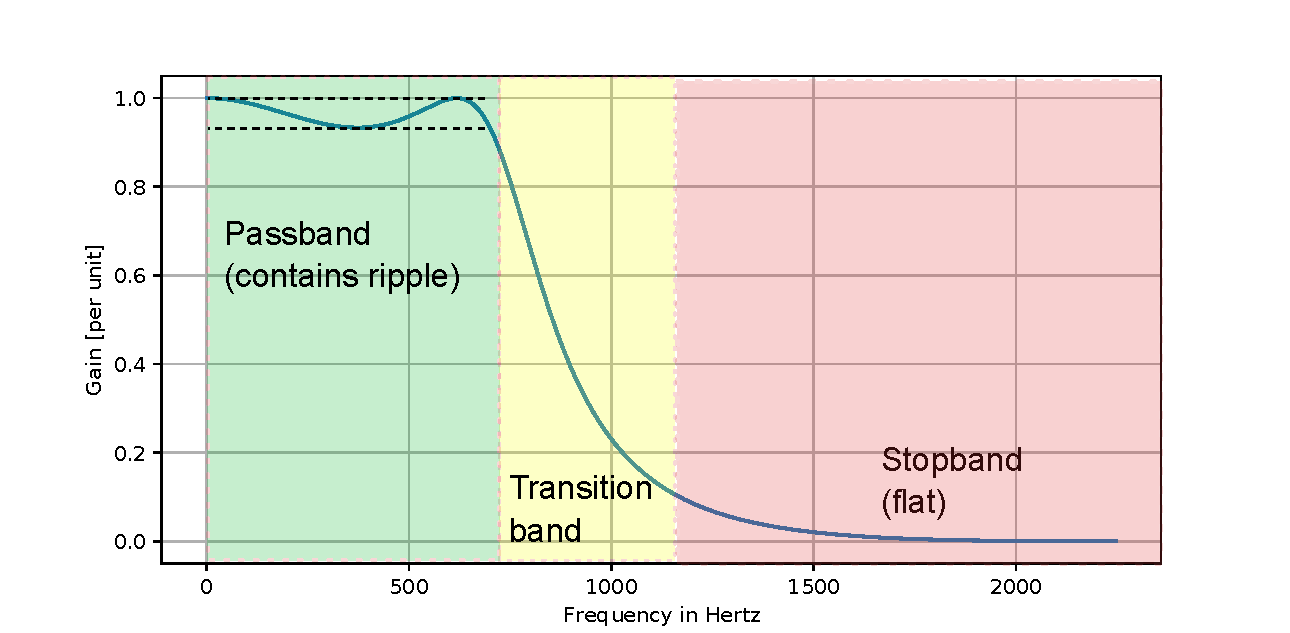
\includegraphics[width=10cm]{graphics/filter_bands/filter_bands_good.pdf}}
%\caption{Example of a frequency response of a non-ideal low-pass filter}
%\label{fig_filter_nonidealities}
%\end{figure}

While obtaining the filter's output for a given frequency range, the Root Mean Square (RMS) value of this output can be simultaneously computed by summing the squares of each sample and taking the square root of the sum. The RMS value can be interpreted as energy content of a signal. Hence, in our concept, we utilize it to represent the intensity of the vibration in the corresponding frequency range \cite{b3}.


% ===============================================================
\subsection{Clustering}
\label{sec_clustering}

As explained in Section \ref{sec_associated_challenges}, industrial machinery usually presents different operational modes. The resulting differences in vibration signals should be considered in the analysis of the acquired signals. In this paper, we apply clustering techniques to identify aggregation patterns in the vibration signals.

In statistical data analysis, the term clustering refers to dividing data points into subgroups, also called clusters, of data points that are considered similar according to some specification. 

In this context, the concept of similarity can be defined in various forms. A simple and intuitive method is the Euclidean distance between the data points, meaning that points located close to each other are considered similar.

This section then describes two specific techniques employed in the clustering task in this work: the K-Means algorithm and the Principal Component Analysis.

\subsubsection{K-Means}

K-Means refers to identifying a certain number of positions around which the data points tend to aggregate themselves and then labeling the data points according to the closest positions of identified aggregation. The objective of K-Means is to find the centroids, which minimizes the Within-Cluster Sum of Square (WCSS), as expressed in Equation \ref{eq_kmeans_wcss}: 

%Figure \ref{fig_kmeans_intuition} provides an intuition for the working principle behind this technique. It illustrates a toy example with multiple datapoints which aggregate themeselves in two clusters. The objective of K-Means is to find points $C_{A}$ and $C_{B}$, namely the centroids, which minimizes the WCSS, which is determined as per expressed in Equation \ref{eq_kmeans_wcss}:

\begin{equation}
	\label{eq_kmeans_wcss}
	WCSS=\sum_{i = 1}^{m} l_{i}^{2}
\end{equation}

Where $m$ is the number of points in the dataset and $l$ is the Euclidean distance between each point $p_{i}$ and the nearest centroid $c_{i}$ to it. For an illustrative two-dimensional example, $p_{i}$ has coordinates $p_{ix}$ and $p_{iy}$, while $c_{i}$ has coordinates $c_{ix}$ and $c_{iy}$, and the corresponding Euclidean distance is expressed in Equation \ref{eq_kmeans_distance}. This expression can then be expanded for an $n$-dimensional space.

\begin{equation}
	\label{eq_kmeans_distance}
	l_{i}=\sqrt{(p_{ix} - p_{ix})^{2} + (p_{ix} - p_{ix})^{2}}
\end{equation}

A method for determining the centroids $c_{i}$ which minimize WCSS is given by Lloyd's algorithm \cite{b3}, which starts with initial guesses for each $c_{i}$ and then, iterativelly, assigns each $p_{i}$ to the neares $c_{i}$, then recalculate each $c_{i}$ as the average position of the $p_{i}$ assigned to it. The process can be terminated when the $c_{i}$'s positions stabilize. Then, the segregation of the data into groups is determined by which centroid each datapoint is associated.

The choice for the K-Means technique stems from the method's simplicity and graphic intuition, which facilitates maintenance teams to analyse the results delivered by the system in order to better plan maintenance schedules. 

%\begin{figure}[htbp]
%\centerline{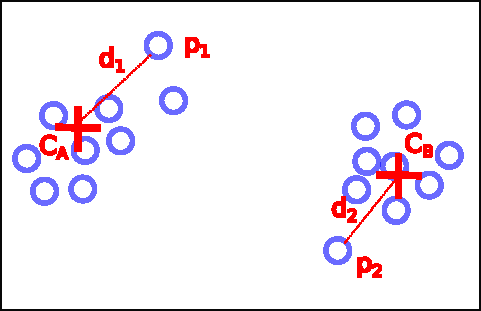
\includegraphics[width=0.5\columnwidth]{graphics/clu_kmeans_intuition.pdf}}
%\caption{Intuition of K-Means clustering technique}
%\label{fig_kmeans_intuition}
%\end{figure}

The K-Means technique does not specify the number of clusters in the data. This information that must be input into the problem. However, it is usually not known beforehand, and figuring out how many clusters the underlying patterns in the data present is part of a data clustering procedure. % The Principal Component Analysis, presented in the next session, comes into play in this task by facilitating that humans apply their expertise to identify patterns visually.

\subsubsection{Principal Component Analysis}

Principal Component Analysis (PCA) is a data dimensionality reduction technique. This enables humans to use their sense of vision to try to find insights into the data by representing the data set in two or three dimensions.

The technique can be explained as applying a change of basis in the data matrix, where the new basis is composed of vectors that point in the directions of maximum variance in the data. These vectors, also called Principal Components, are hierarchically sorted based on how much of the total data variance they explain.

Such principal component vectors are equivalent to the eigenvectors of the data's covariance matrix, and the variance explained by them is directly related to their associated eigenvalues \cite{b7}. Thus, the math behind PCA can be summarized by building a linear transformation matrix with the eigenvectors of the covariance matrix and then applying this linear transformation to the data in question.

The data's covariance matrix $C$, of dimensions $m \times m$, where $C$ is given as per Equation \ref{eq_pca_covmatrix}:

\begin{equation}
	\label{eq_pca_covmatrix}
	C=\frac{1}{m}\sum_{i = 1}^{m}(x^{(i)}-\mu)(x^{(i)}-\mu)^{T}   
\end{equation}

where $x^{i}$ denotes the row-wise vector of the dimension $i$ in the data set, and must represent the mean of the dimension vector. 

% ===============================================================
\subsection{Anomaly Detection}
\label{sec_anomaly_detection}
Anomaly Detection (AD) refers to diverse mathematical techniques that aim to detect outliers in datasets. These techniques can be summarized to comprise the following steps: 

\begin{enumerate}
	\item Providing a mathematical model that captures the underlying patterns in a data set.
	\item Using this model to declare if a given data point conforms to the model-associated pattern or not, that is, if it is a normal or an anomalous point.
\end{enumerate}

In our concept, we apply Multi-Variate Gaussian Distribution (MVGD), where the data points have more than one dimension. In addition, we determine the probability that the point belongs to the distribution, considering the correlation of the variables in the data.

This calculation is performed based on the covariance matrix $C$, already presented in Equation \ref{eq_pca_covmatrix}. The probability of data point $x$ is given by Equation \ref{eq_mvg_mvg}:

\begin{equation}
	\label{eq_mvg_mvg}
	p(x|\mu,C)=\frac{1}{(2\pi)^{n/2}|C|^{1/2}}\exp{\left(\frac{1}{2}(x-\mu)^{T}C^{-1}(x-\mu)\right) }
\end{equation}

By applying Equation \ref{eq_mvg_mvg}, the "normality level" of a given observation can be directly associated with the resulting probability. For applications like quality control, an AD technique can be implemented using a threshold to each sample's probability level and rejecting the ones below the threshold. For vibration-based predictive maintenance, however, observing the variation of the vibration measurements probability over time is more beneficial. This approach gives an indication of the deterioration of the machine's health over time.

Fig. \ref{fig_mvg_singlecaseinnadequade} provides a graphical illustration of anomaly detection. Obviously, point $x_{anom}$ does not conform to the pattern displayed by the other points, i.e., $x_{anom}$ represents an anomaly. By analyzing $x_{anom}$'s coordinates $x_{1}$ and $x_{2}$ separately, the anomaly is not evident, as the coordinates are well within the range defined by the other points. However, by focusing on the correlation between $x_{1}$ and $x_{2}$ by means of the distribution's covariance matrix, the MVGD assigns $x_{anom}$ a much lower probability than the other points.

\begin{figure}[htbp]
\centerline{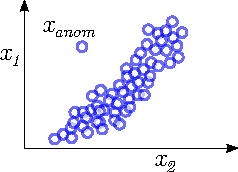
\includegraphics[width=0.3\columnwidth]{graphics/single_variab_innadequate.pdf}}
\caption{Illustration of anomaly that single variate Gaussian anomaly detection strategy fails to detect}
\label{fig_mvg_singlecaseinnadequade}
\end{figure}

Regarding the application of the MVGD for a given data set, a caveat is that meaningful results can be obtained if the dimensions of the data set are gaussian-distributed. Dimensions that present high mean and median differences are generally not suitable for MVGD. Nevertheless, in this case, it is possible to apply statistical transforms to map the original distribution to the one that is more gaussian-shaped. One such transformation is the Quantile Transform, which integrates the quantile regression technique to estimate the gaussian cumulative distribution of the variable \cite{koenker2001quantile}.


% ===============================================================
% ===============================================================
% ===============================================================
\section{Hardware Implementation - Data Aquisition Setup}
\label{sec_implementation}

The vibration monitoring hardware and software infrastructure (see Fig. \ref{concept_pre}) used in this work was developed by the company DELTA Systems GbR and is installed in a textile manufacturing plant in the city of Malatya in Turkey. The hardware setup comprises a set of 85 wireless vibration sensors, which are all installed in the same machine and communicate via two gateways over the radio.

The wireless electronic sensors are embedded systems controlled by a microcontroller. The program is written in C language, and the compiled machine code is stored in the microcontroller. The system also comprises an external flash memory to store vibration measurements for later analysis and/or transmission. 

A significant challenge related to the operation of the sensors is their energy autonomy. Since these sensors are designed to be placed in a compact case, the space available for their battery supply is quite limited. From this perspective, it is required to ensure that energy-intensive operations, such as radio communication, are used as little as possible.

The gateway modules are embedded computers with a Linux operational system. They run an application written in Python, responsible for interacting with a SQLite database, communicating with the field sensors over radio, and providing a graphical user interface that can be accessed via TCP/IP based connection from a desktop computer connected to the same network. 

\begin{figure}[htbp]
\centerline{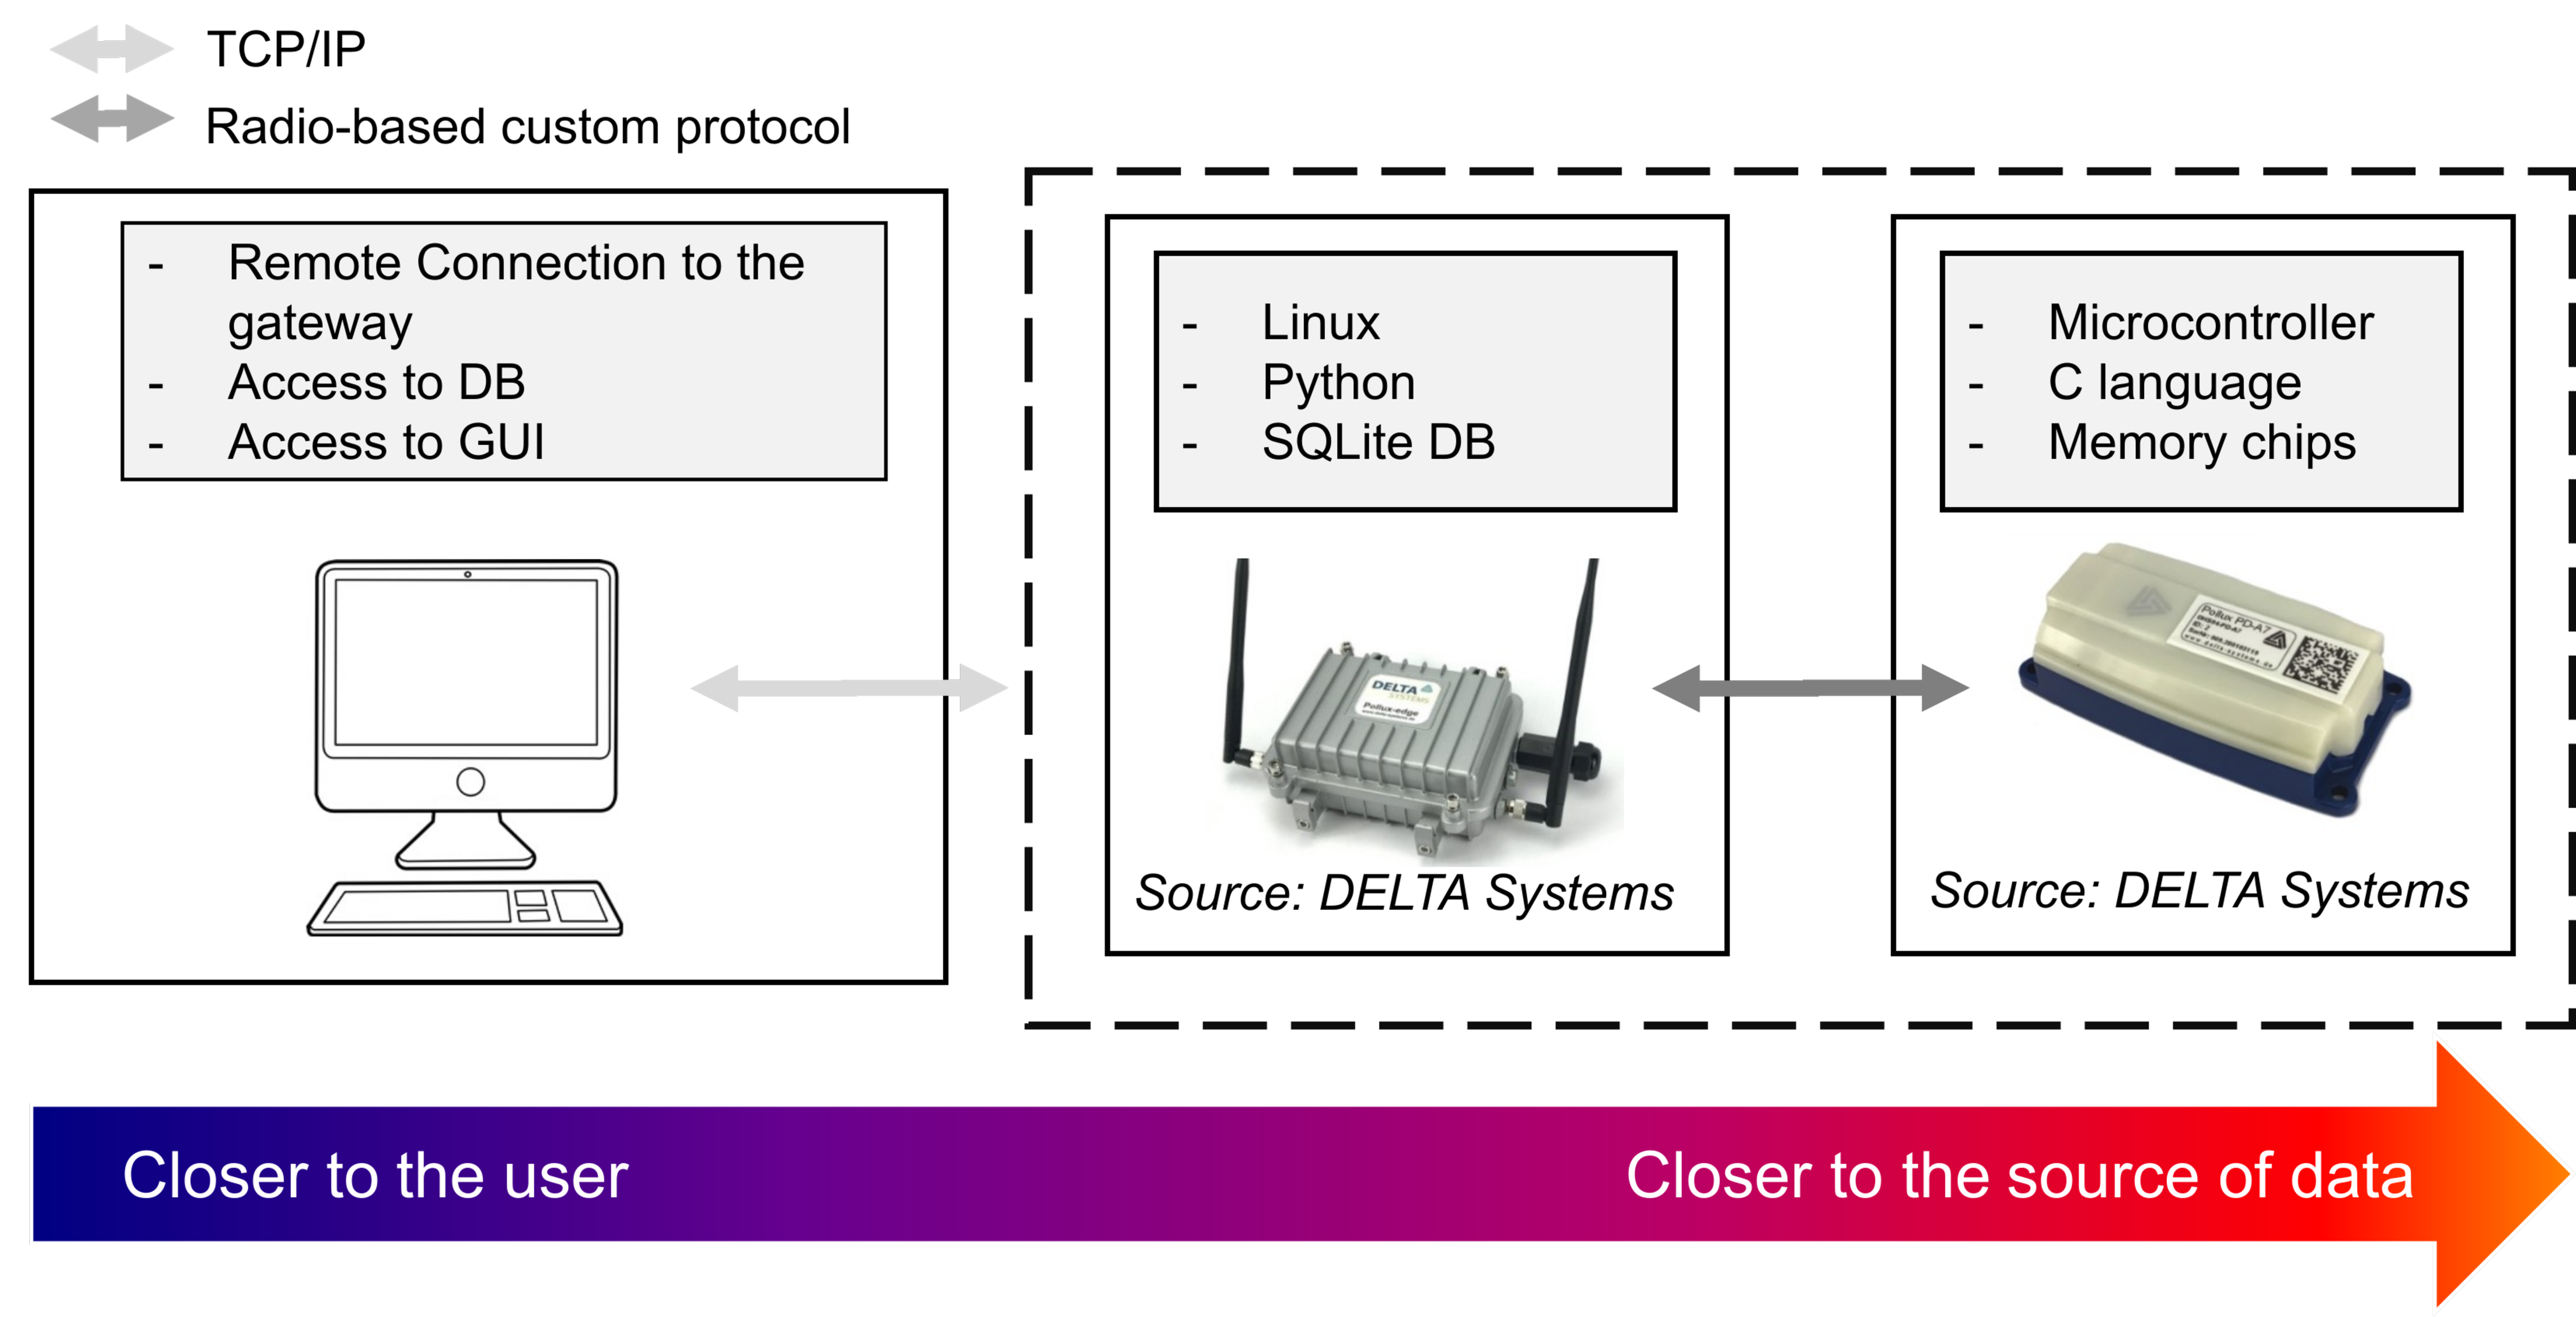
\includegraphics[width=\columnwidth]{graphics/concept/concept_pre_new.pdf}}
\caption{An Overview of the system's architecture}
\label{concept_pre}
\end{figure}

% ===============================================================
% ===============================================================
% ===============================================================
\section{Results and Discussion}
The concept is implemented at all 85 sensors installed at the machine. Hence, in this section, we select and present the results derived from one of those sensors and initiate our discussion. 
\label{sec_results_discussion}
% ===============================================================
\subsection{Data Exploration - Overview of the vibration measurements}

The electronic sensors provide vibration measurements along the three Cartesian axes $x$, $y$, and $z$, with origin and orientation to the package of the digital vibration transducer integrated circuit. We let the fictional axis $a$ be defined as $a = \sqrt{x^{2}+y^{2}+z^{2}}$. This fictional axis $a$ contains all the frequency components found in $x$, $y$, and $z$. An example of a measured signal is presented in Fig. \ref{fig_example_signals}.

\begin{figure}[htbp]
\centering
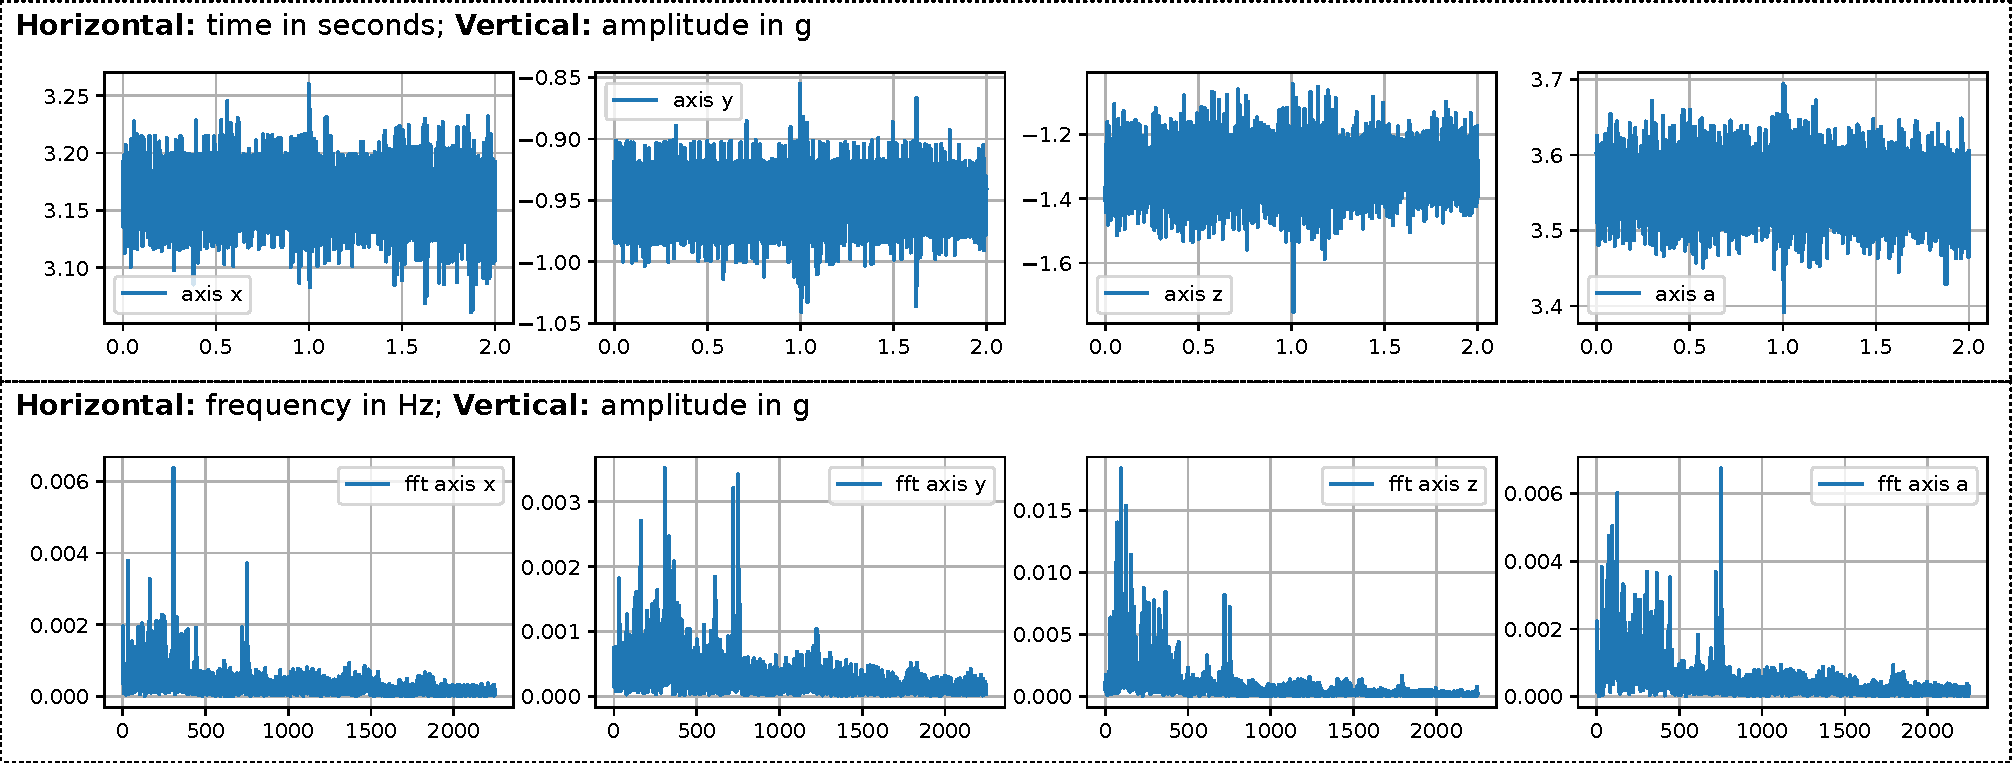
\includegraphics[width=\columnwidth]{graphics/axes_time_fft/axes_time_fft.pdf}
\caption{Plot of an example of a vibration signal over axes $x$, $y$, $z$ and $a$, on both time (top) and frequency (bottom) domain}
\label{fig_example_signals}
\end{figure}

On the firmware side, the vibration measurements are configured to a sampling frequency of 4500Hz and duration of 2s. Hence, the number of samples for each axis in a measurement is $N=4500Hz \cdot 2s = 9000$. The frequency resolution results in $\Delta f = 4500Hz/9000 = 0.5 Hz$, using Equation \ref{eq_freq_resolution}.

% ===============================================================
\subsection{Machine Speed}
\label{sec_machine_speed}

In order to obtain from the vibration measurements an indication of the machine's operating speed, we look more closely into a certain frequency range, including a peak. Since the wider the range, the more calculations according to $k$ are required. For the range from 25Hz to 35Hz, we can theoretically as well as experimentally observe a peak. Hence, we look more closely into this frequency range. A plot for this specific region for different $a$-axis measurement signals is presented in Fig. \ref{fig_motor_frequency}. The result indicates that, in this range, there is sometimes a peak near 30 Hz, and sometimes there is no discernible peak at all. 

An important takeaway from this observation is the confirmation that the rotating frequency $f_{motor}$ can be obtained in the 25 to 35 Hz range, which allows us to restrict the expensive FT calculations accordingly. In other words, in the FT computations in Equation \ref{eq_fourier_disc}, the calculations are performed only for the $k$-indexes from $25Hz/\Delta f = 50$ to $35Hz/\Delta f = 70$.

As for the measurements with no discernible peak in the observed region, they presumably represent measurements acquired when the machine was not operating; see Section \ref{sec_clustering_results}.

\begin{figure}[htbp]
\centerline{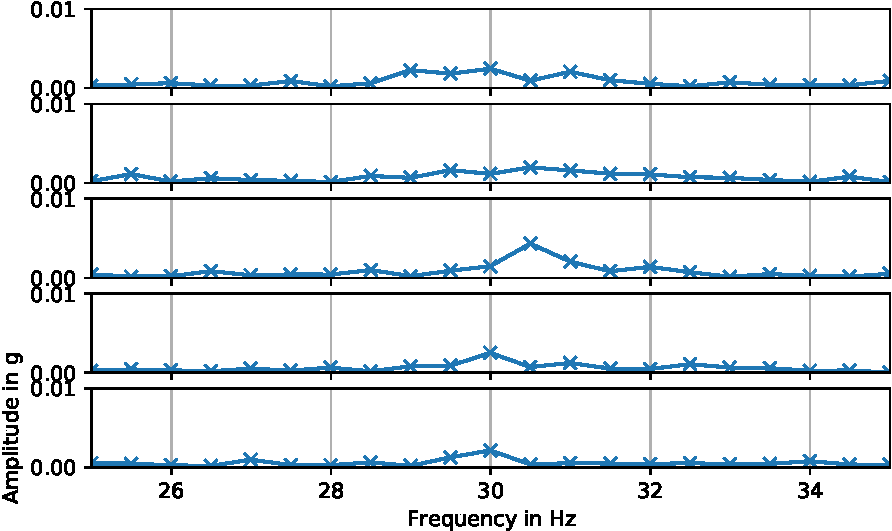
\includegraphics[width=\columnwidth]{graphics/motor_frequency/motor_frequency_ohne.pdf}}
\caption{Observations of the $a$-axis frequency spectra in the expected range for $f_{motor}$}
\label{fig_motor_frequency}
\end{figure}



% ===============================================================
\subsection{Digital Filters}

In the introduction to Section \ref{sec_signal_processing}, we presented three vibration signal's characteristics of our interest in the analysis: 1) the machine's speed $f_{motor}$, which can be calculated as explained in Section \ref{sec_machine_speed}, 2) the energy content of the vibration signal, which can be easily obtained by the RMS value of the $a$-axis of the measurement, and 3) the distribution of the vibration's energy over its frequency spectrum. Section \ref{sec_digital_filters_concept} proposes an instruction to acquire the third one with reasonable computational cost by computing the RMS values of the output of digital filters.

For this purpose, the available frequency range of up to 2250Hz (according to the Nyquist theorem with a sampling frequency of 4500Hz) is divided into three subranges:

\begin{itemize}
	\item a lower range up to 500 Hz
	\item a middle range between 500 and 1250 Hz
	\item a higher range from 1250 Hz on
\end{itemize}

The higher the number of ranges, the more detailed the vibration energy distribution over frequency, at the cost of more computations required.

For each of these ranges, a digital filter is developed. These filters are named, in a notation based on their discrete-time transfer functions, as $F_{low}$, $F_{mid}$ and $F_{high}$, according to their associated frequency range. Considering Section \ref{sec_digital_filters_concept}, the main design decisions are summarized as follow:

\begin{itemize}
	\item \textbf{Topology}: We select the inverse Chebyshev as the topology. The first reason for this choice is the narrow transition band, which is always desirable. The trade-off for the narrower transition band is a larger phase distortion, which is irrelevant for our case, as we do not consider a phase in our modeling. Finally, we desired a flat passband in order to preserve the information as much as possible for our modeling.
	\item \textbf{Order}: As a general rule, the overall performance of the filter is improved with higher order, at the cost of more computations required. By experimentation, the	trade-off order should be set to 3.
	\item \textbf{Overlap}: Some overlap is included in the cutoff frequencies of the three filters. This is a decision taken to achieve an optimum configuration within the numerous trade-offs in filter design. Hence, $F_{low}(z)$ was defined as a low-pass with cutoff at 700 Hz, $F_{mid}(z)$ was defined as a band-pass with cutoff at 400 and 1350 Hz, and $F_{high}(z)$ as a high-pass at 1150 Hz.
\end{itemize}

Consequently, we give the $a$-axis signal of the vibration measurements as input (see Fig. \ref{fig_filters_example_inout}, left ) and present the output of these transfer functions (see Fig. \ref{fig_filters_example_inout}, right). The output in frequency domain (right bottom) proves that the filters work as expected since the output from the filters gathers in the corresponding frequency region. It is noted that the filter $F_{high}$ catches practically a lot of lower frequency contamination, as the lower frequencies own relatively higher intensity. The resulting problem can be solved by increasing the order of the filter.  

%\begin{figure}[htbp]
%\centerline{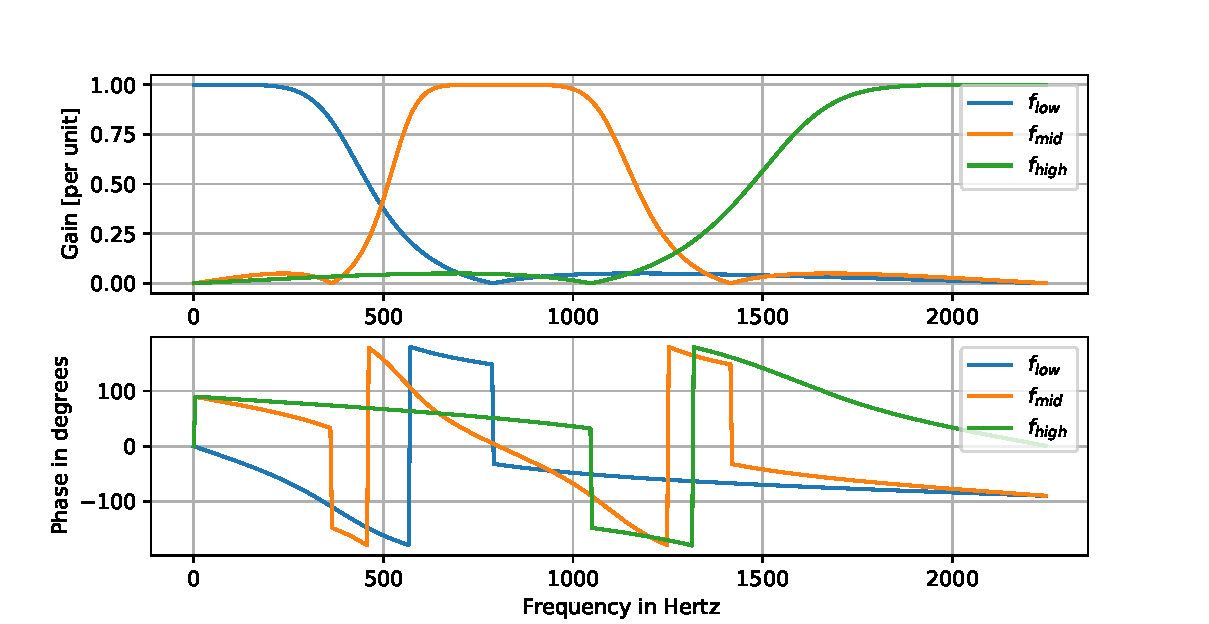
\includegraphics[width=\columnwidth]{graphics/filters_freqresponse/filters_freqresponse.pdf}}
%\caption{Frequency response of the three filters}
%\label{fig_filters_freq_response}
%\end{figure}

\begin{figure}[htbp]
\centering
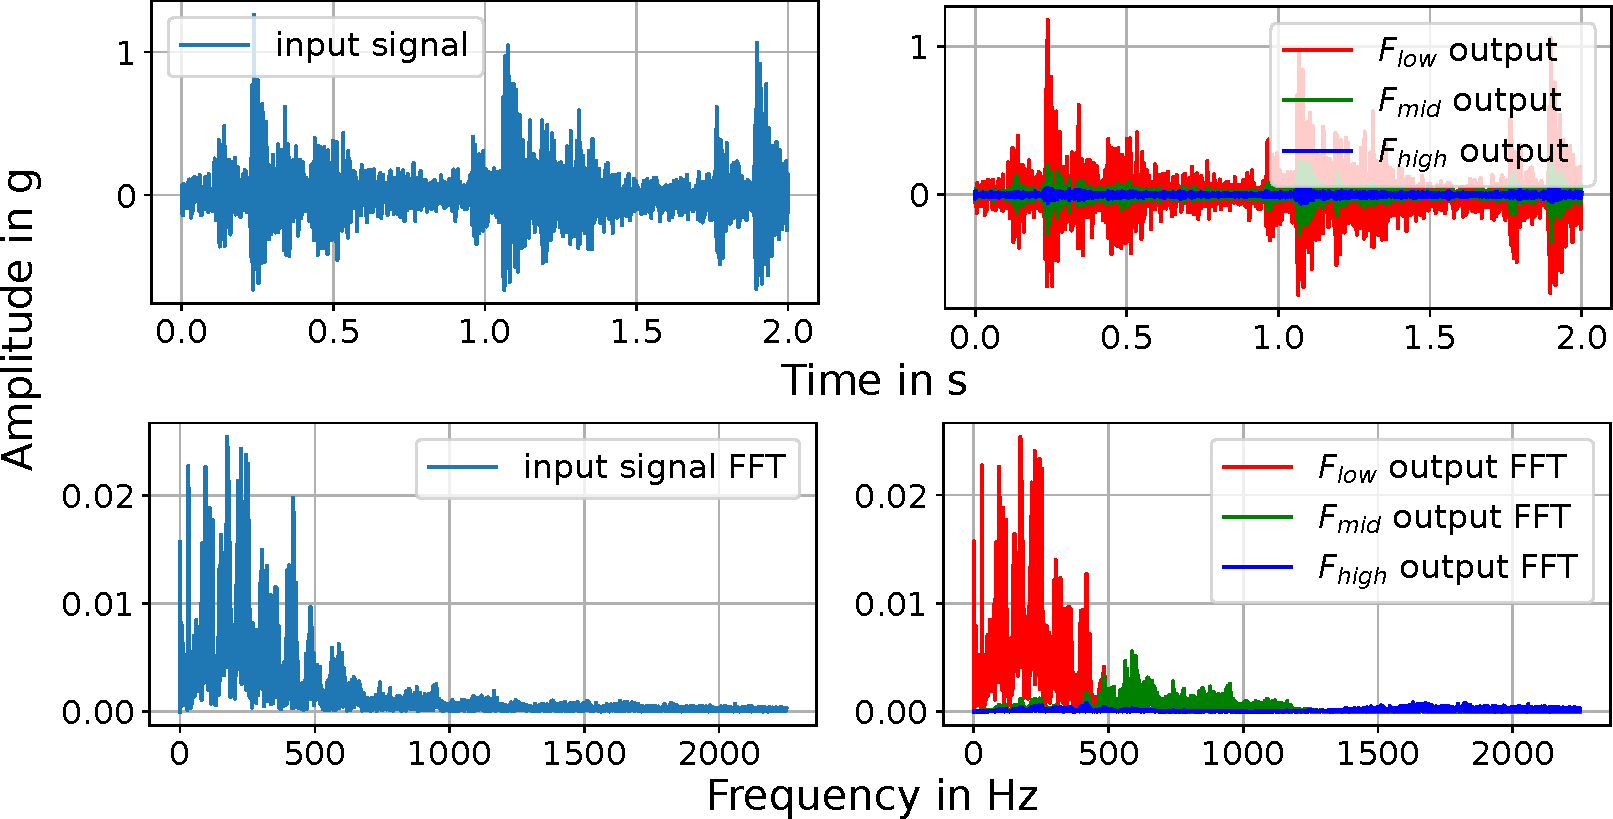
\includegraphics[width=\columnwidth]{graphics/filters_sigresponse/filters_sigresponse_ohne.pdf}
%\centerline{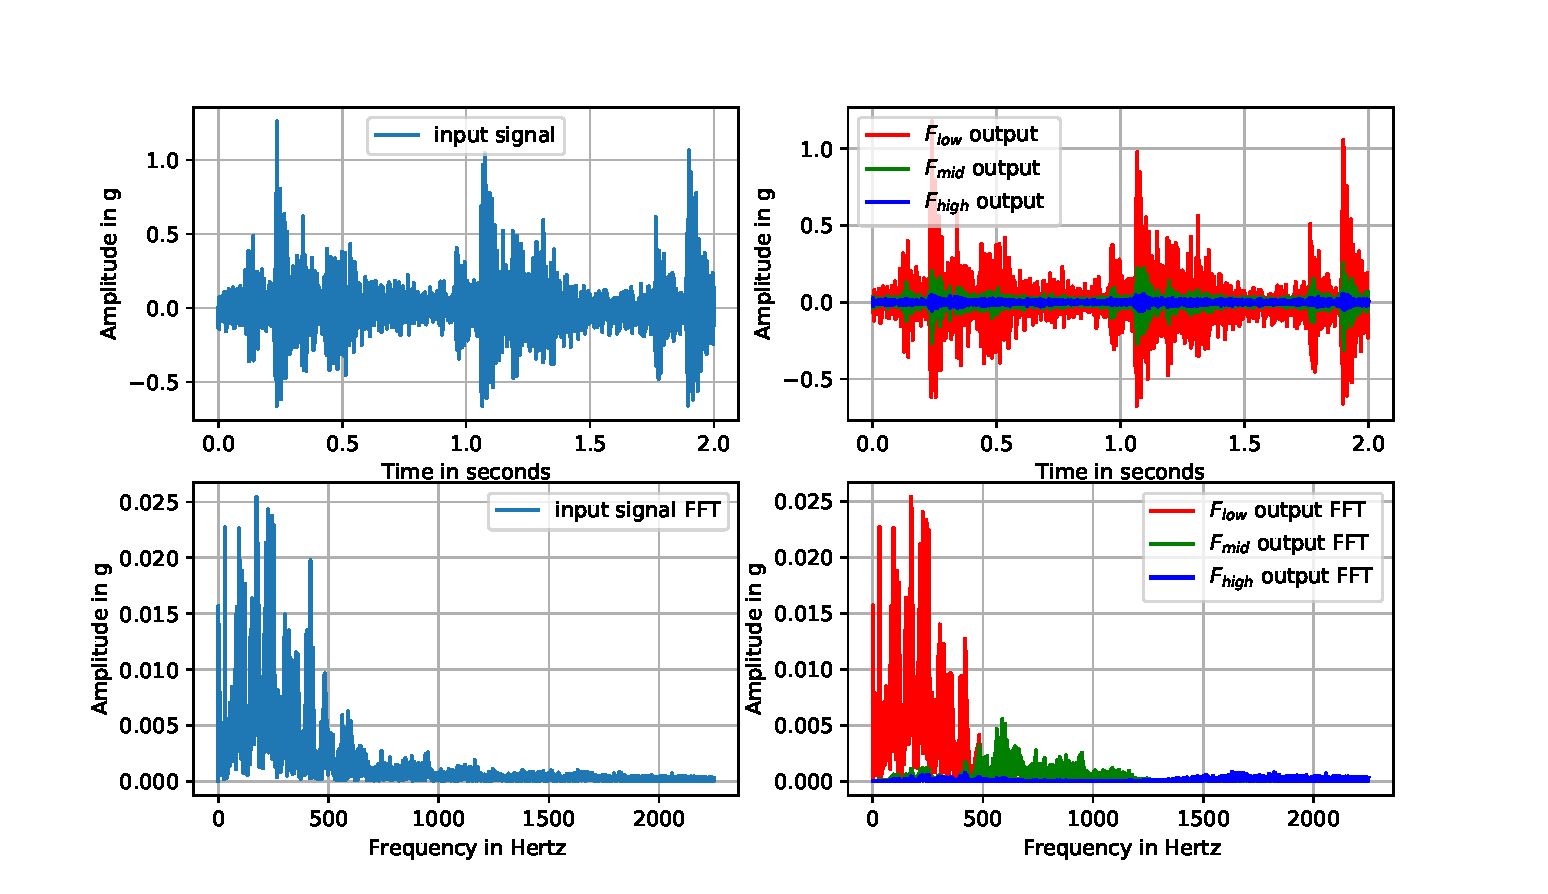
\includegraphics[width=\columnwidth]{graphics/filters_sigresponse/filters_sigresponse.pdf}}
\caption{Observation of filters' output in time and frequency domain based on an $a$-axis measurement}
\label{fig_filters_example_inout}
\end{figure}



% ===============================================================
\subsection{Clustering: Segregation of Operational Modes}
\label{sec_clustering_results}

In order to understand the underlying patterns in the data, the first step refers to performing Principal Component Analysis on the data set. The input to this analysis is comprised of five features:

\begin{itemize}
	\item $f_{motor}$: peak frequency in the 25Hz to 35 Hz range
	\item $RMS_{total}$: RMS value of the $a$ axis
	\item $RMS_{low}$: RMS value of the output of the $F_{low}(z)$ filter
	\item $RMS_{mid}$: RMS value of the output of the $F_{mid}(z)$ filter
	\item $RMS_{high}$: RMS value of the output of the $F_{high}(z)$ filter
\end{itemize}

The resulting PCA plot is presented in Fig. \ref{fig_pca_result}. This same plot also shows a segregation of the points based on the results of a Kmeans clustering procedure.


\begin{figure}[htbp]
\centerline{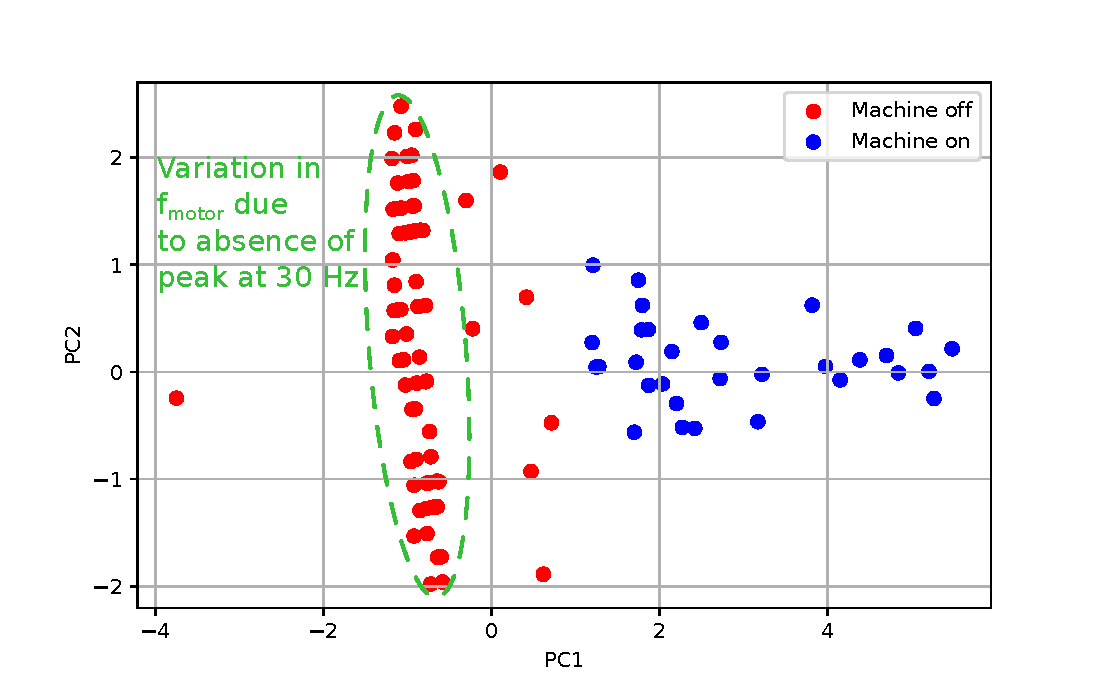
\includegraphics[width=0.9\columnwidth]{graphics/pca_result/pca_result.pdf}}
\caption{PCA plot for the described dataset}
\label{fig_pca_result}
\end{figure}

While analyzing the measurements assigned to each cluster, it was noted that one of the clusters was characterized by lower vibration levels in general than the other one. Hence, we can conclude that the former represents the "operational" state while the machine is off, and the later while the machine is on. This conclusion is supported by the region with large variation, encircled in a green dashed shape. When the machine is off, the motors are not running, so they do not produce the 30 Hz peak. Thus, the peak in the range from 25Hz to 35Hz ends up being mostly randomly defined by noise.

When the machine is off, its vibration signature is of low relevance for PM. Thus, the analysis focuses on the cluster representing the machine in its "on" state. The segregation can be easily carried out by the $RMS_{total}$ value. This threshold value is set to $0.015g$. At this point, it is worth to mention that the $a$ axis signal has its average value removed, so the $1g$ gravity vibration is not present in the signal.

% ===============================================================
\subsection{Approach to Anomaly Detection}
At the current data analysis stage, the data is already clustered, and a single cluster was selected for further analysis. Thus, the variability left in the data is expected not to result in multimodal distributions for a given variable. In order to implement the MVGD-based AD strategy discussed in Section \ref{sec_anomaly_detection}, it is required that the variables are Gaussian-distributed. In order to ensure that, we apply the quantile transform to the data. Fig. \ref{fig_transform_result} depicts the variables before and after the transformation.

% \begin{figure}
% 	\centering
% 	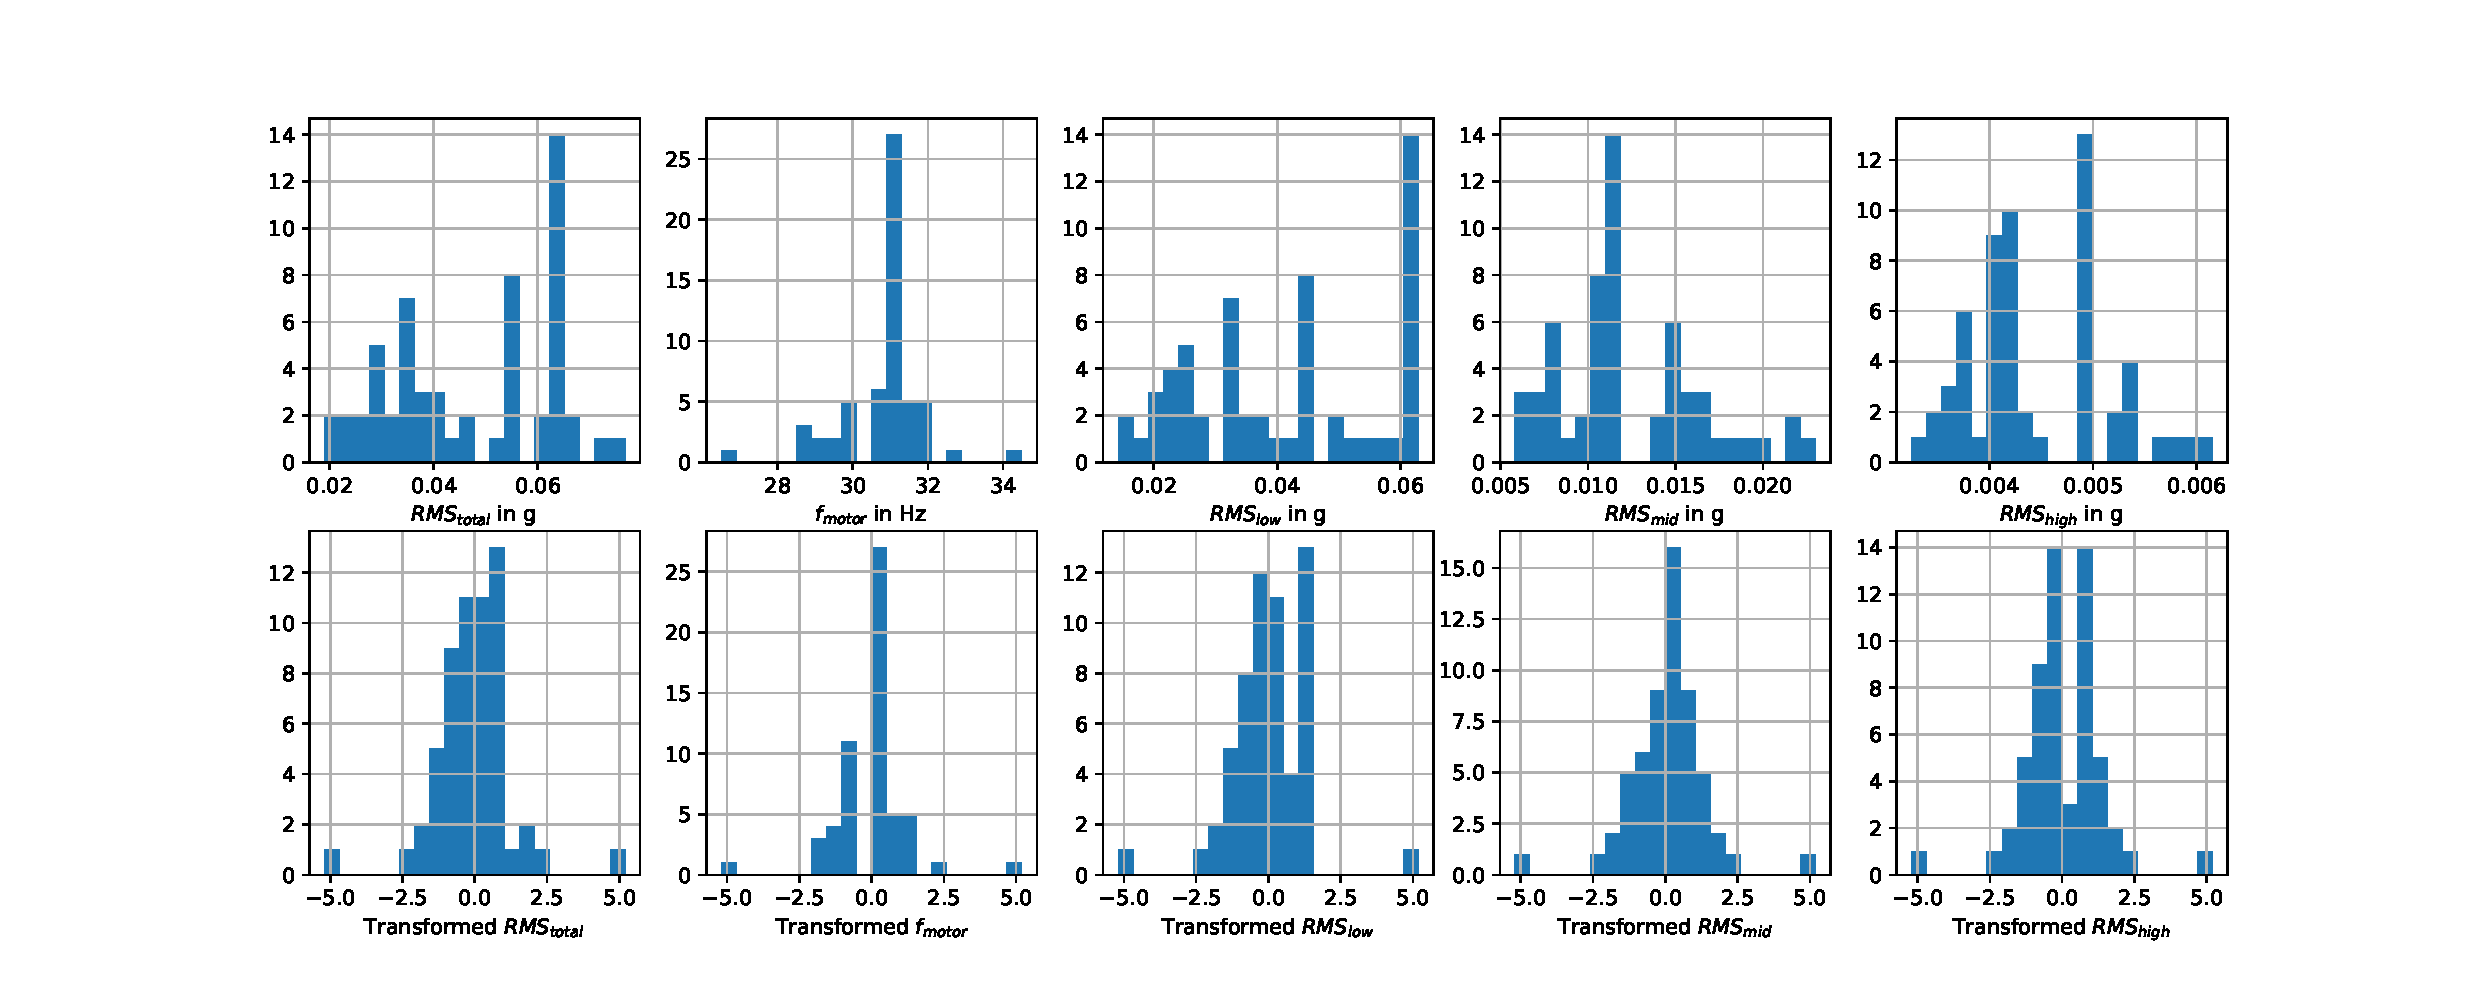
\includegraphics[width = \textwidth]{quantile_transform_data/quantile_transform_data.pdf}
% 	\caption[Transformed data]{Variables before and after quantile transform}
% 	\label{fig_transform_result}
% \end{figure}

\begin{figure}[htbp]
\centerline{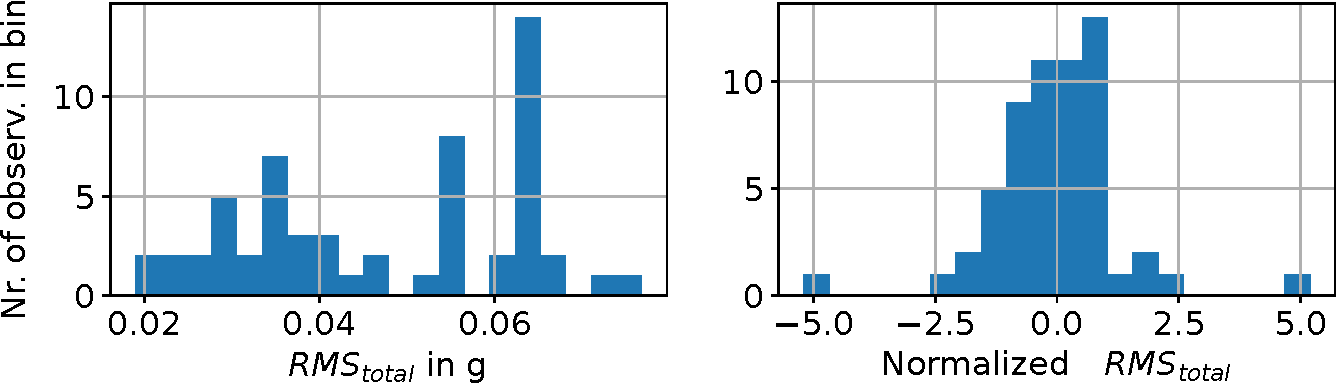
\includegraphics[width=\columnwidth]{graphics/quantile_transform_data/quantile_transform_data_ohne.pdf}}
\caption{Variables before and after quantile transform}
\label{fig_transform_result}
\end{figure}

For the actual AD approach, it is decided to build a concept based on the evaluation of the MVGD probability for four distinct models:

\begin{enumerate}
	\item Covariance between $f_{motor}$ and $RMS_{total}$
	\item Covariance between $f_{motor}$, $RMS_{total}$ and $RMS_{low}$
	\item Covariance between $f_{motor}$, $RMS_{total}$ and $RMS_{mid}$
	\item Covariance between $f_{motor}$, $RMS_{total}$ and $RMS_{high}$
\end{enumerate}


Fig. \ref{fig_mvgd_plot} represents the measurement points' associated probability derived from the proposed four covariance models previously defined. In this 3D heatmap representation, the $x$ and $y$ axes represent, respectively, the transformed $f_{motor}$ and RMS value(s). At the same time, the resulting normality level, highlighted in the heatmap color, represents the measurement points' associated probability. As the color gets darker, the normality is lower. Hence, if a new points  derived from a specific sensor keeps being darker, the intervention of a technician is required to investigate the parts in the region where this sensor is attached. 

% \begin{figure}
% 	\centering
% 	\includegraphics[width = \textwidth]{mvgd_plots/plot1_fmotor_rmstotal.pdf}
% 	\caption[MVGD plot for $f_{motor}$ and $RMS_{total}$]{MVGD plot for $f_{motor}$ and $RMS_{total}$}
% 	\label{fig_mvgd_plot1}
% \end{figure}

%\begin{figure}[htbp]
%\centerline{\includegraphics[width=\columnwidth]{graphics/mvgd_plots/plot1_fmotor_rmstotal.pdf}}
%\caption{MVGD plot for $f_{motor}$ and $RMS_{total}$}
%\label{fig_mvgd_plot1}
%\end{figure}

\begin{figure} 
    \centering
  \subfloat[\label{1a}]{%
       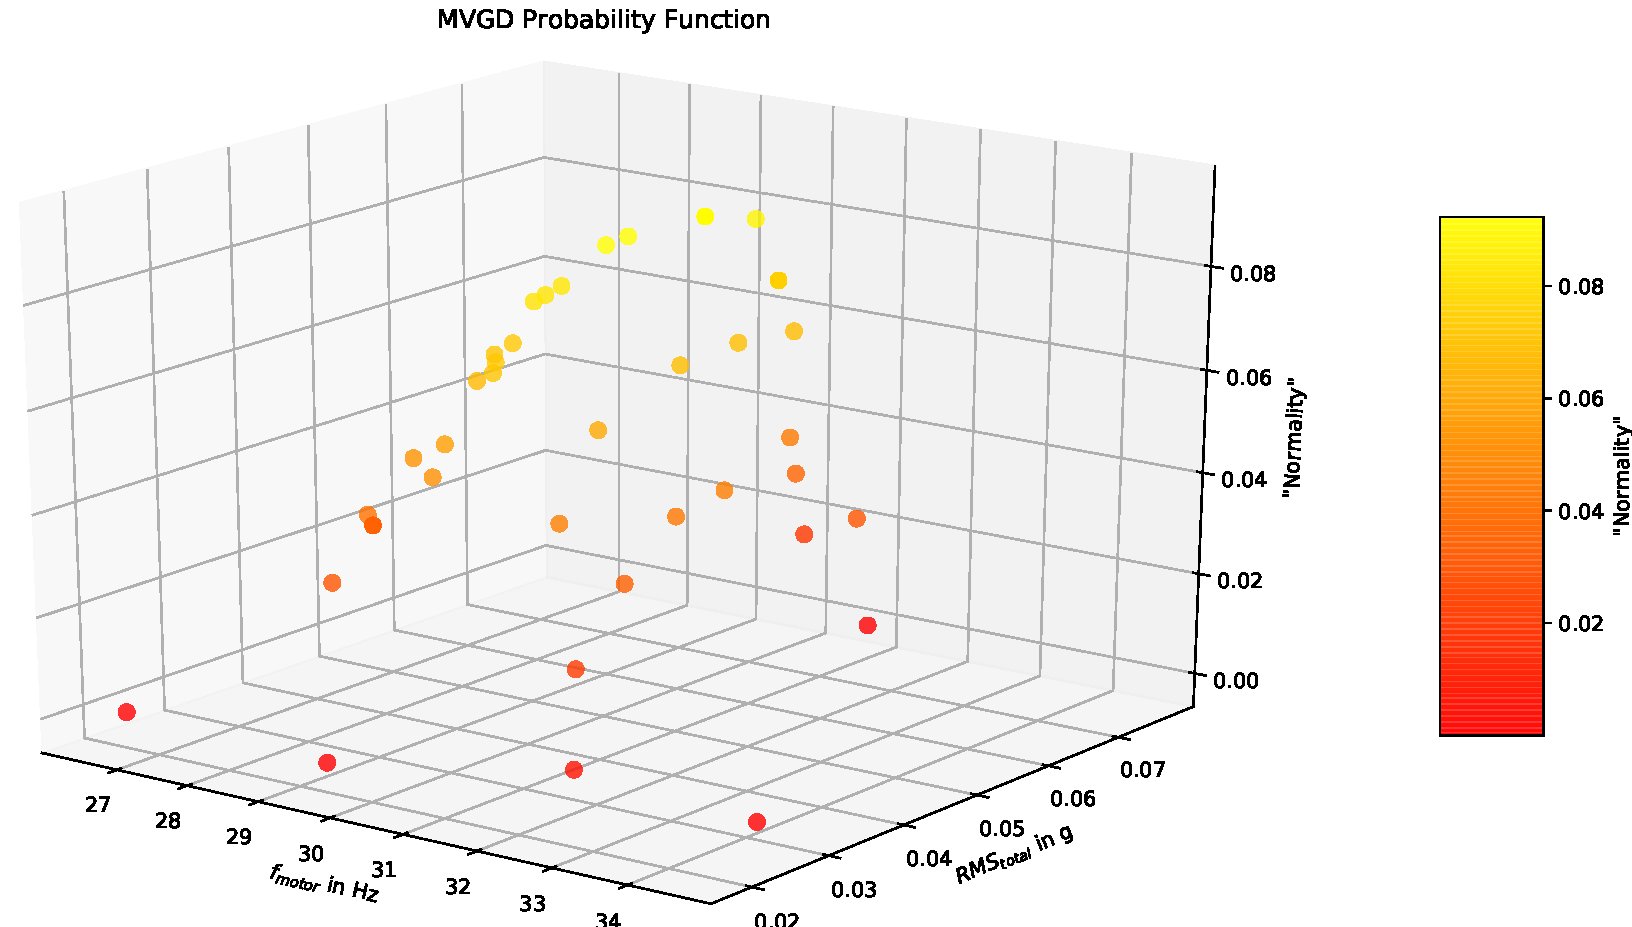
\includegraphics[width=0.5\linewidth]{graphics/mvgd_plots/plot1_fmotor_rmstotal_ohne.pdf}}
    \hfill
  \subfloat[\label{1b}]{%
        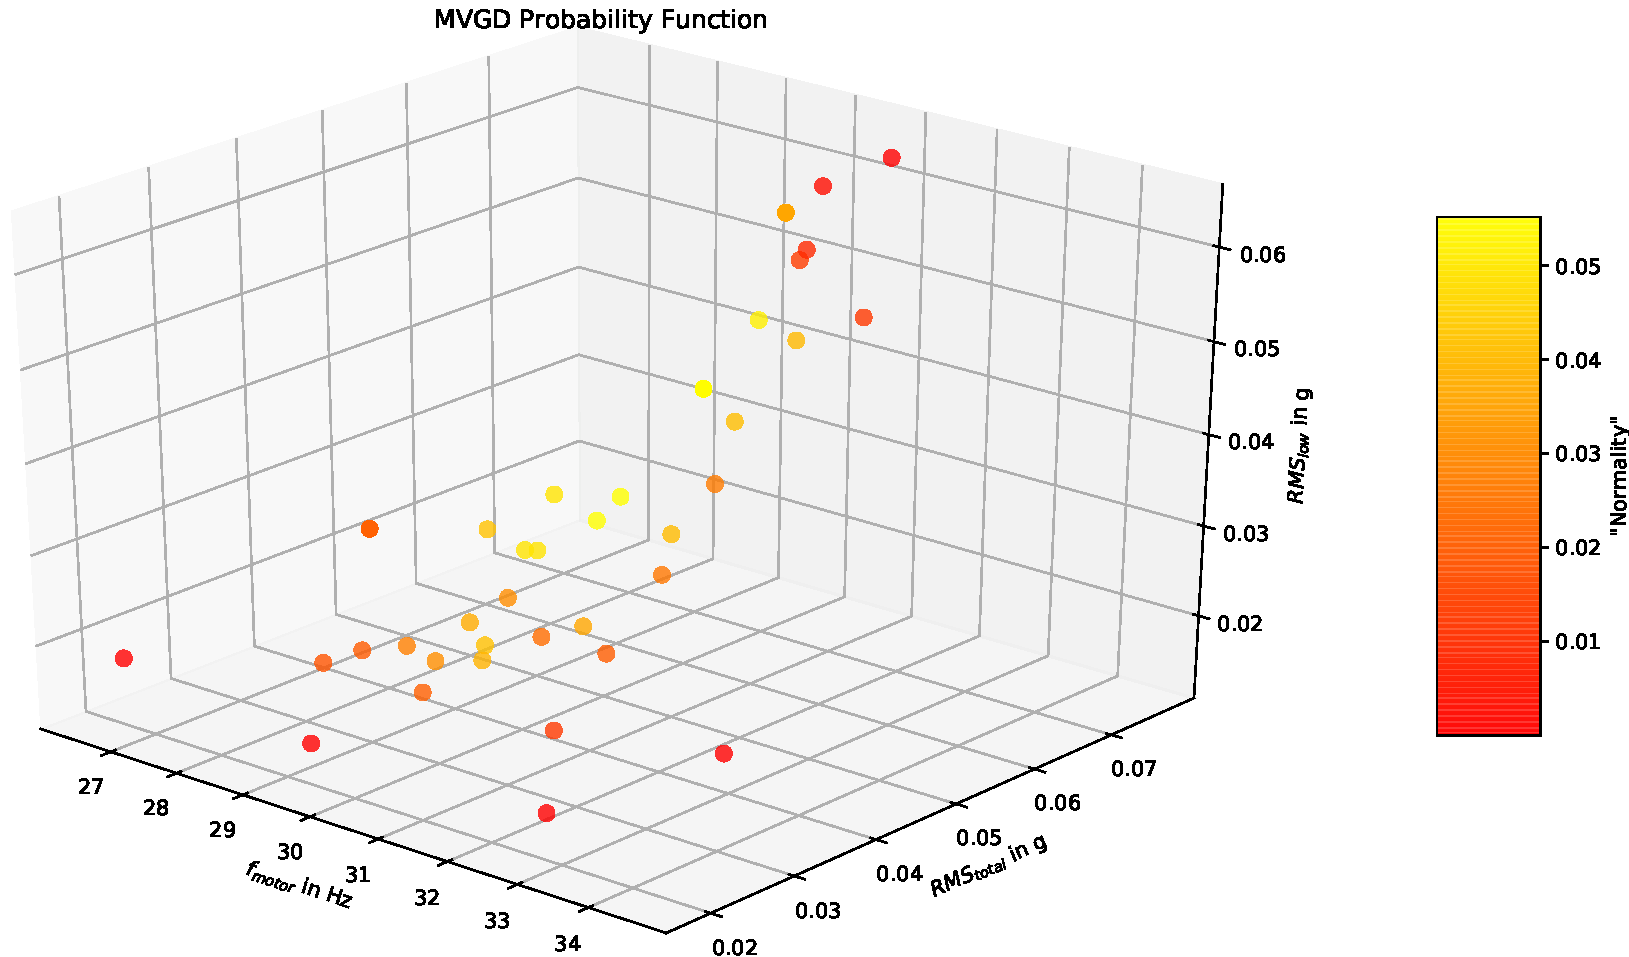
\includegraphics[width=0.5\linewidth]{graphics/mvgd_plots/plot2_fmotor_rmstotal_rmslow_ohne.pdf}}
    \\
  \subfloat[\label{1c}]{%
        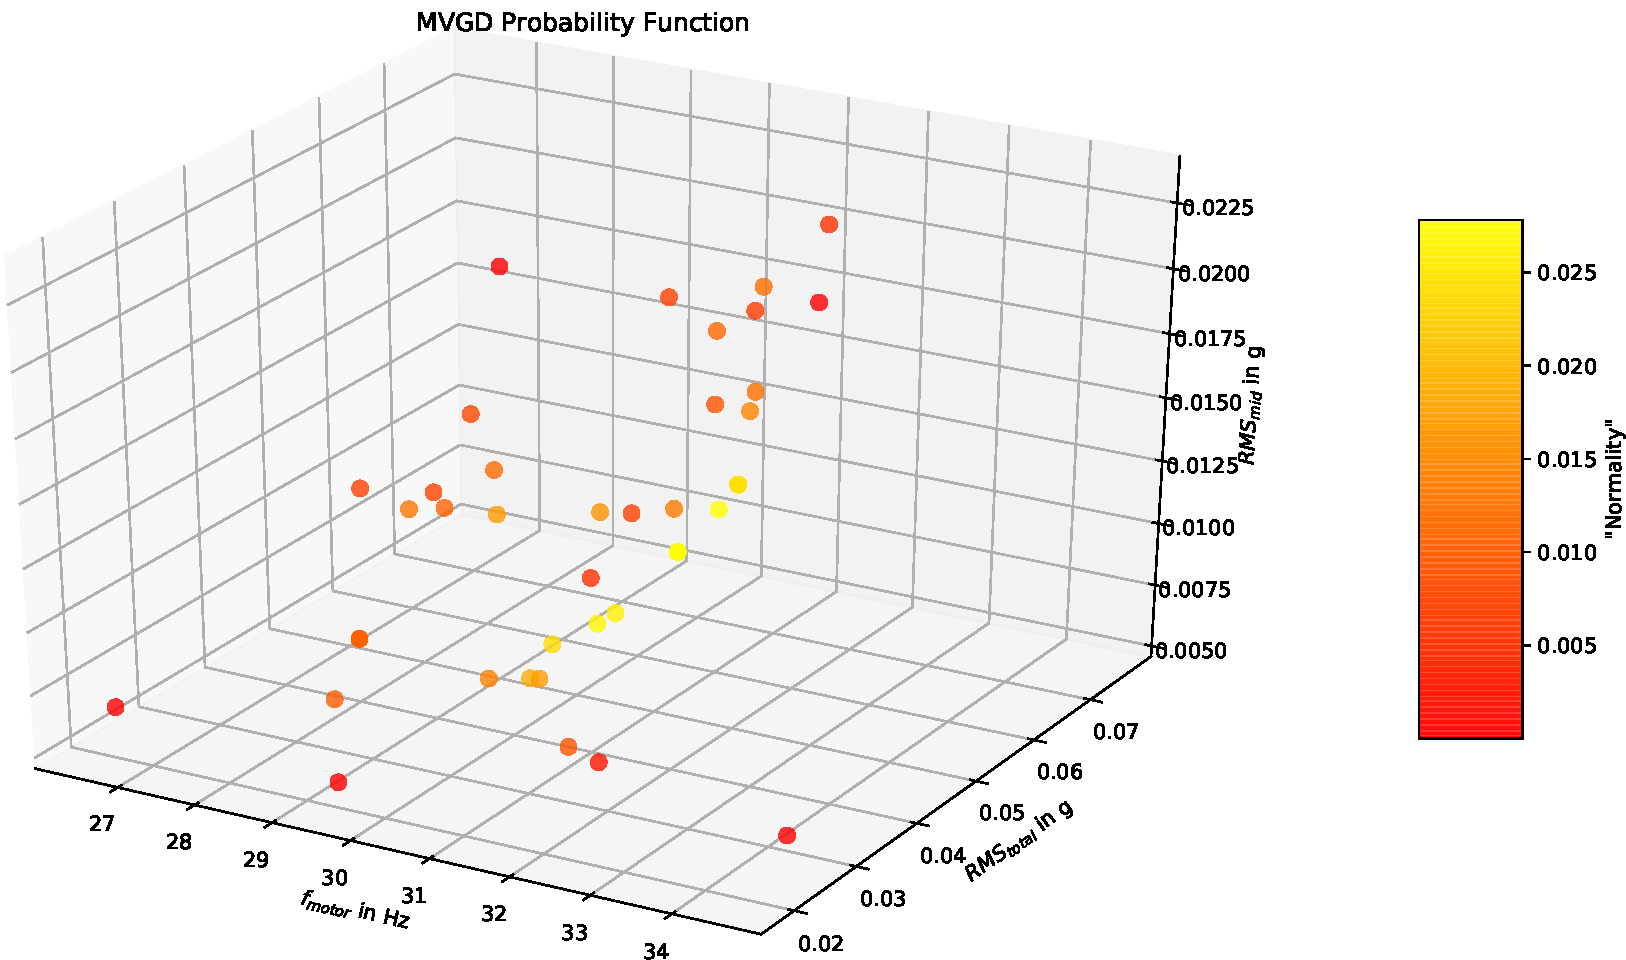
\includegraphics[width=0.5\linewidth]{graphics/mvgd_plots/plot3_fmotor_rmstotal_rmsmid_ohne.pdf}}
    \hfill
  \subfloat[\label{1d}]{%
        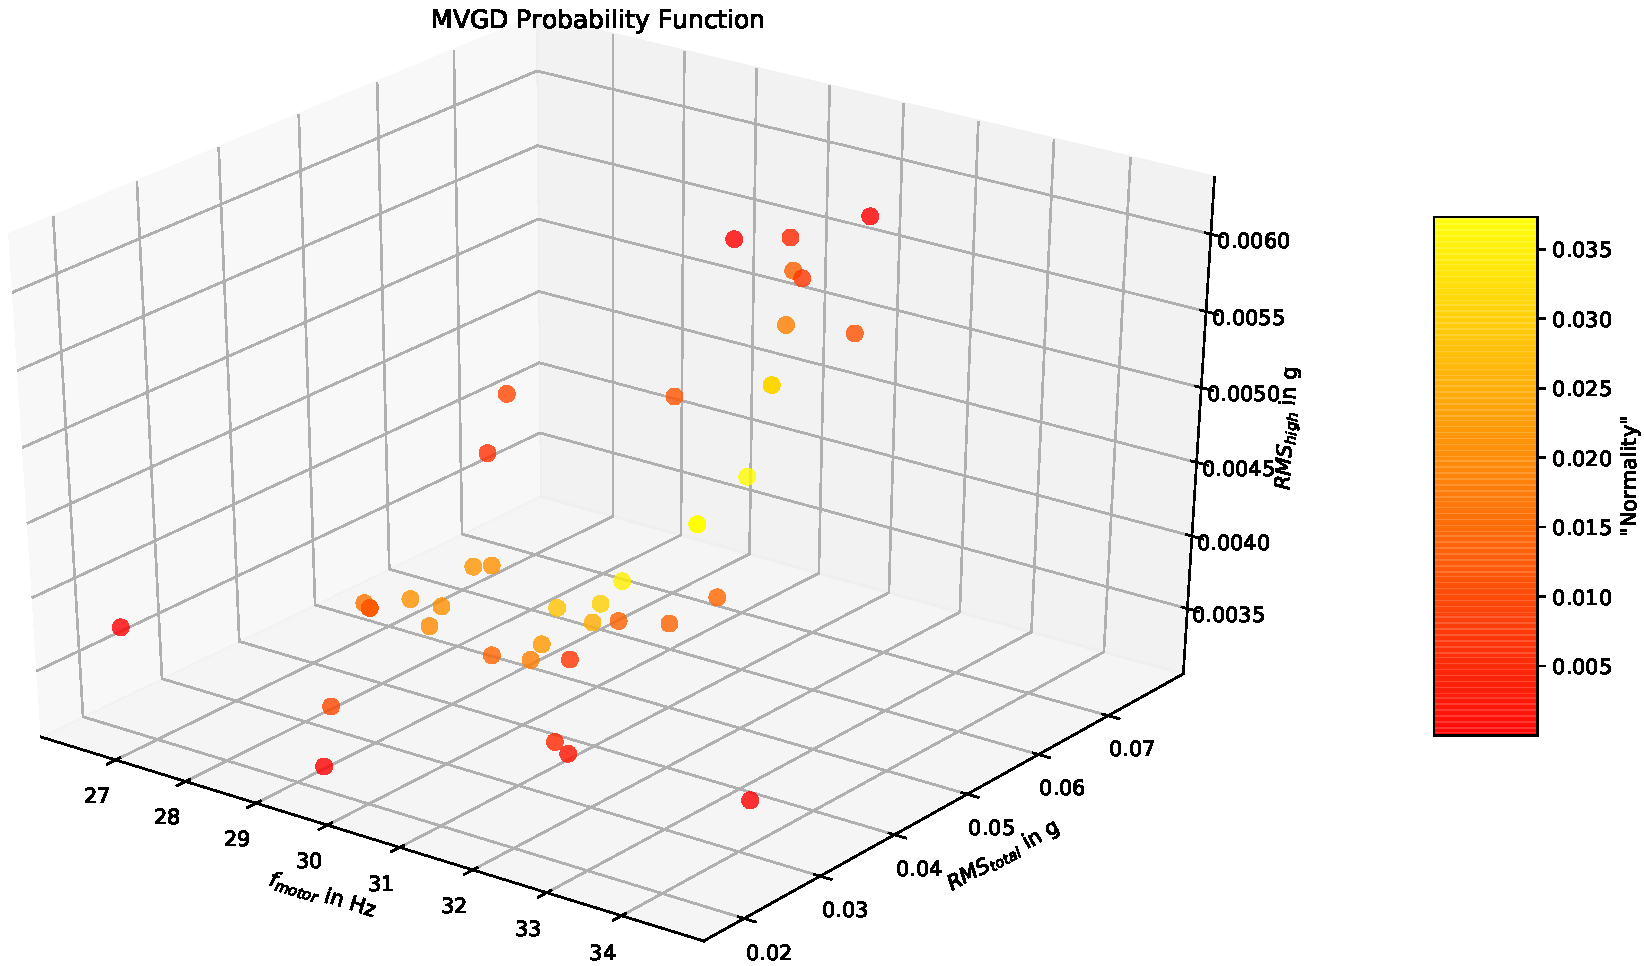
\includegraphics[width=0.5\linewidth]{graphics/mvgd_plots/plot4_fmotor_rmstotal_rmshigh_ohne.pdf}}
  \caption{MVGD plot illustration the four proposed covariance models, respectively (a) the first model for $f_{motor}$ and $RMS_{total}$, (b) the second one for $f_{motor}$, $RMS_{total}$ and $RMS_{low}$, (c) the third one for $f_{motor}$, $RMS_{total}$ and $RMS_{mid}$, and (d) the last model for $f_{motor}$, $RMS_{total}$ and $RMS_{high}$}
  \label{fig_mvgd_plot} 
\end{figure}



%\begin{figure}
%\centering
%\caption{MVGD plot for the proposed four covariance models}
%\label{fig_mvgd_plot}
%\subfigure[Top: the first covariance model between $f_{motor}$ and $RMS_{total}$ Bottom: the second covariance model between  $f_{motor}$, $RMS_{total}$ and $RMS_{low}$]{
%\begin{minipage}[b]{0.2\textwidth}
%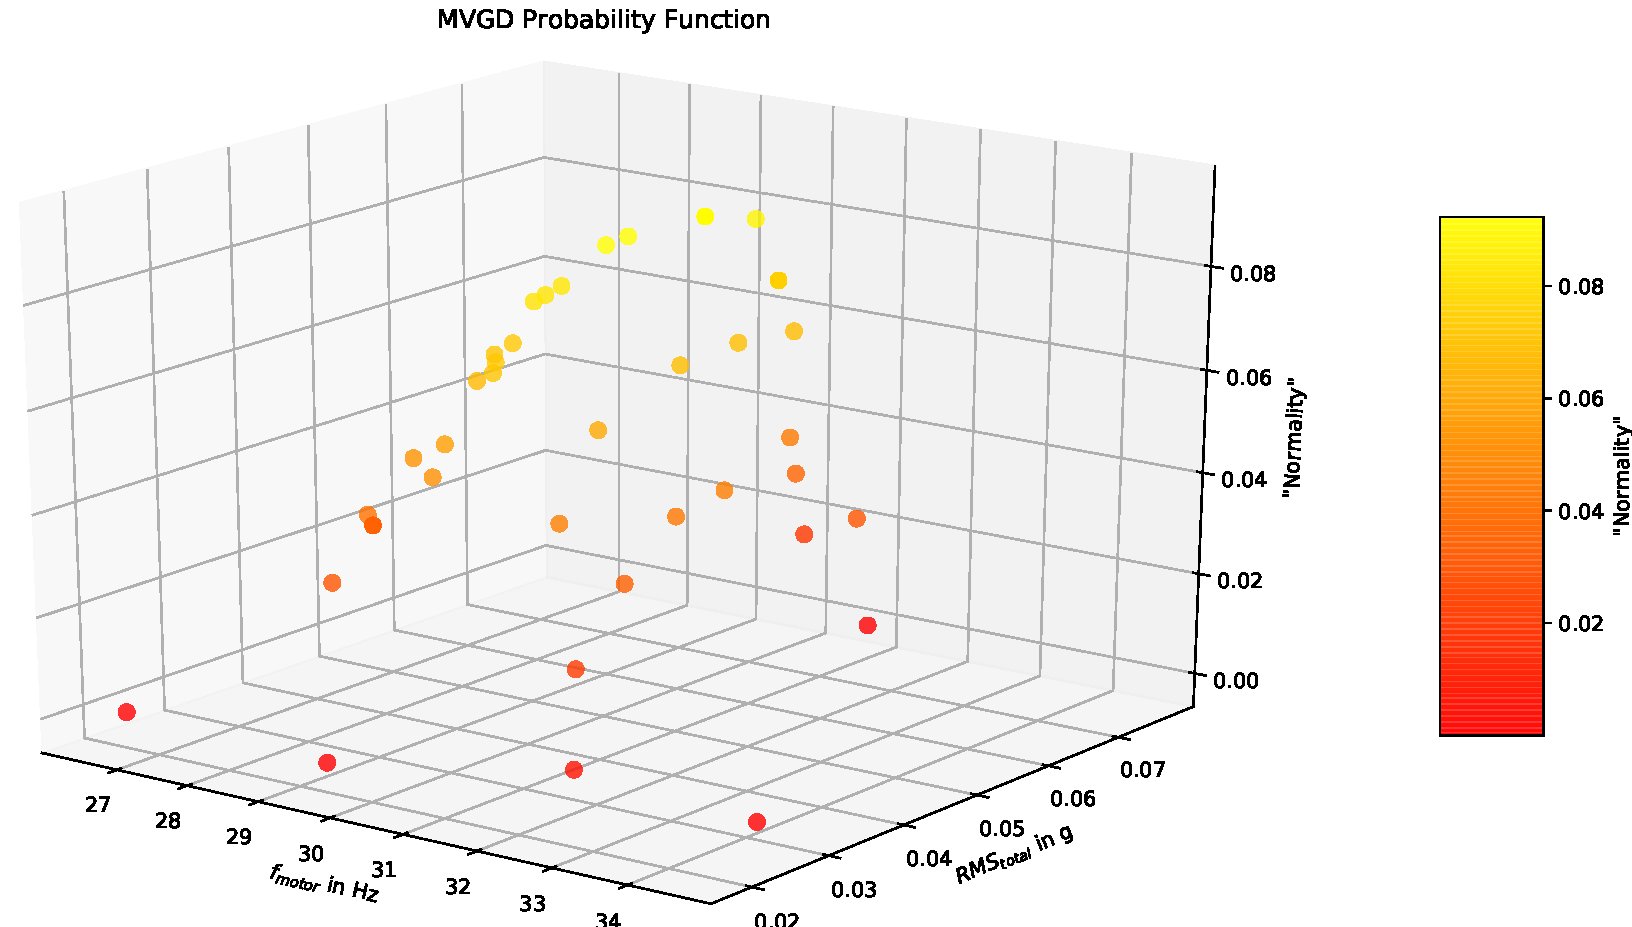
\includegraphics[width=1\textwidth]{graphics/mvgd_plots/plot1_fmotor_rmstotal_ohne.pdf} \\
%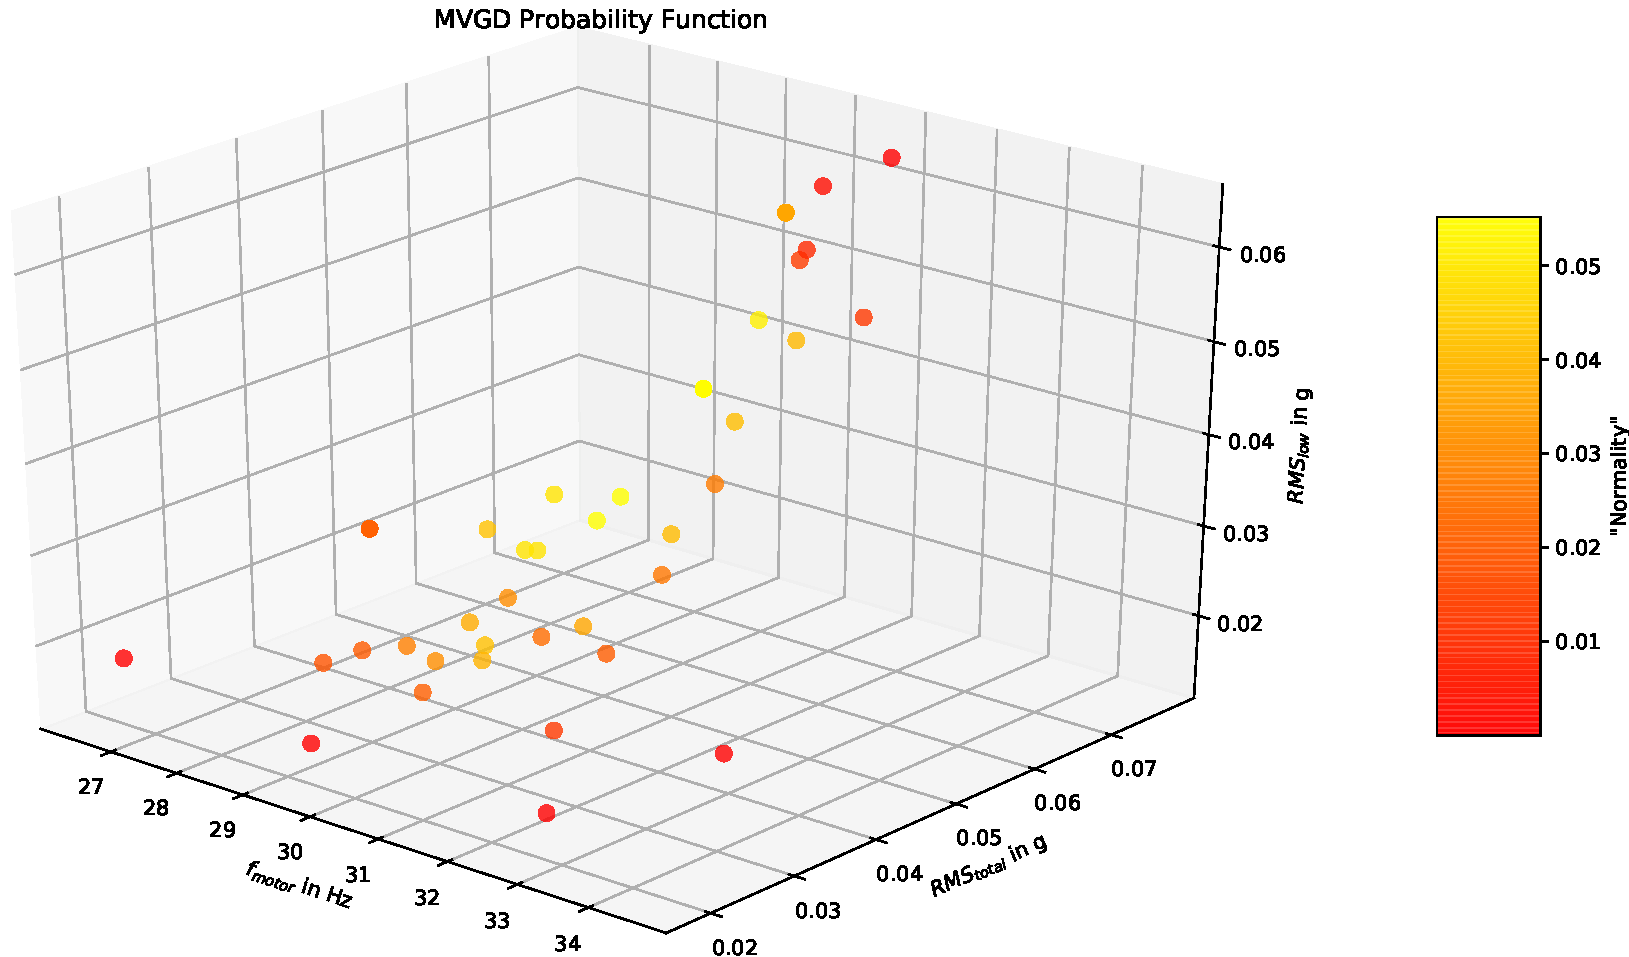
\includegraphics[width=1\textwidth]{graphics/mvgd_plots/plot2_fmotor_rmstotal_rmslow_ohne.pdf}
%\end{minipage}
%}
%\subfigure[the second subfigure]{
%\begin{minipage}[b]{0.2\textwidth}
%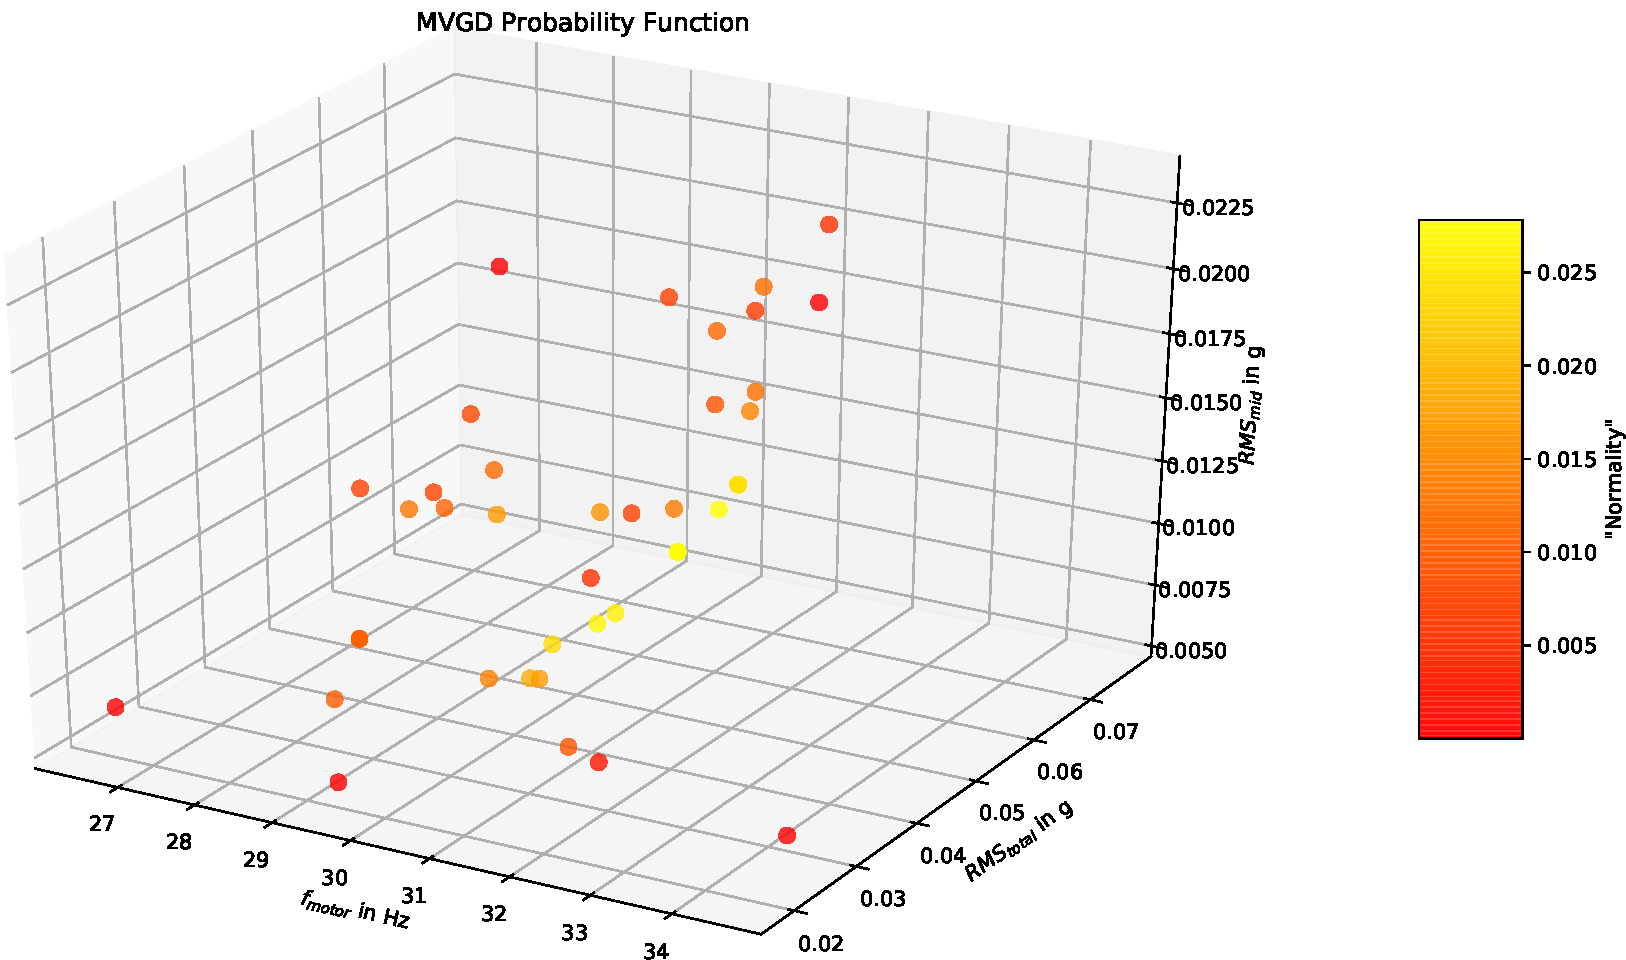
\includegraphics[width=1\textwidth]{graphics/mvgd_plots/plot3_fmotor_rmstotal_rmsmid_ohne.pdf} \\
%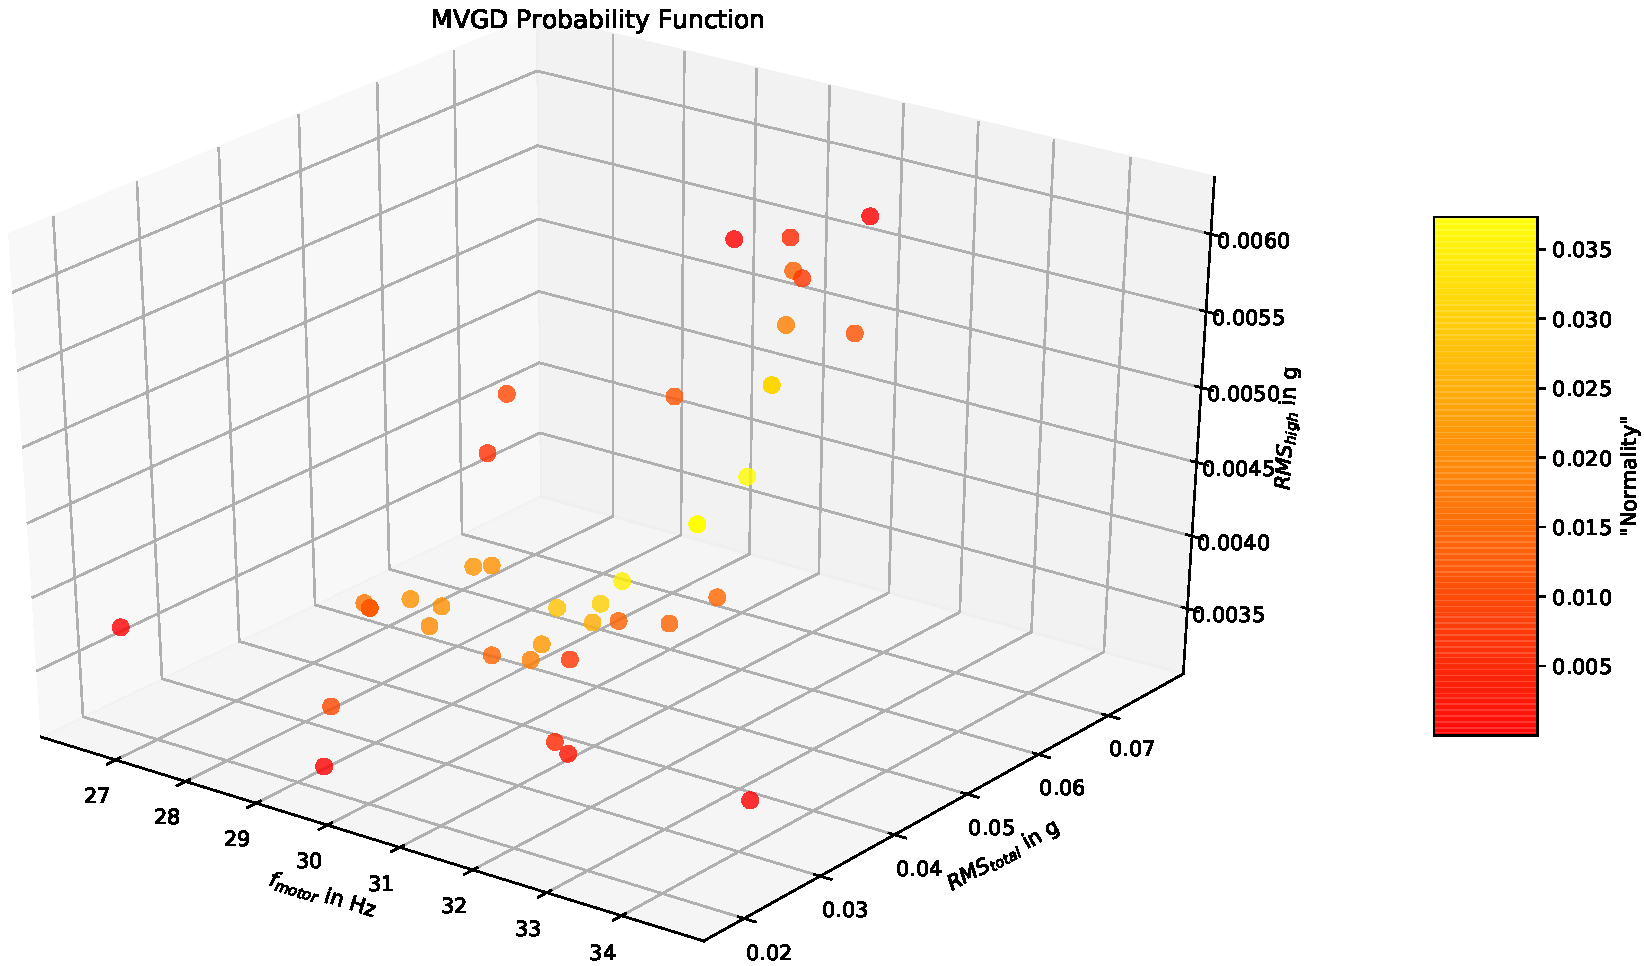
\includegraphics[width=1\textwidth]{graphics/mvgd_plots/plot4_fmotor_rmstotal_rmshigh_ohne.pdf}
%\end{minipage}
%}
%\end{figure}

%The "normality" values for the four covariance models designed are then tracked over time in days in \ref{fig_controlchart_all}. As it can be seen in the plots, it is, unfortunately, not possible to establish a significant deterioration trend or any clearly alarming anomaly. The main cause for this problem is the fact that there are long periods of time without available measurements. With additional data regularly aquired, it should be possible to detect trends more clearly.


% \begin{figure}
% 	\centering
% 	\includegraphics[width =\textwidth]{control_charts/control_chart_v02.pdf}
% 	\caption[Time-evolution of the "normality" values]{Time-evolution of the "normality" values for the different covariance models designed }
% 	\label{fig_controlchart_all}
% \end{figure}

%\begin{figure}[htbp]
%\centerline{\includegraphics[width=\columnwidth]{graphics/control_charts/control_chart_v02.pdf}}
%\caption{Time-evolution of the "normality" values for the different covariance models designed}
%\label{fig_controlchart_all}
%\end{figure}


% ===============================================================
\subsection{Energy Consumption}

The primary consumer of battery energy in the sensors is the radio module. Hence, transmitting less data directly results in less power consumption and, thus, longer battery life. In the previous system, the sensors send the measurement signals entirely. Oppositely, by optimized implementations of the proposal exposed here, the sensor is able to extract the desired features from the measurement data in the edge device and then send only the features by radio. The sum of data bytes transmitted for one measurement is calculated by Equation \ref{eq_energy_consumption_byte}:

\begin{equation}
\begin{aligned}
	N_{b} &= 4500 \cdot  \frac{samples}{second} \times 2 \cdot seconds \times 3 \cdot \frac{axes}{sample} \times 2 \cdot \frac{bytes}{axis} \\
	  &= 54 kbytes
\end{aligned}
\label{eq_energy_consumption_byte}
\end{equation}

A radio message in the protocol has 48 bytes of payload. The vibration sensor needs 30$ms$ to transmit such a message while drawing 18$mA$ at 6$V$. The energy required for each byte is represented by: 

\begin{equation}
\begin{aligned}
	E &= \frac{6V \cdot 18mA \cdot 30ms}{message} \times \left( 48 \cdot \frac{bytes}{message} \right)^{-1} \\
	  & \approx 67.5 \mu Ws/byte
\end{aligned}
\label{eq_energy_consumption_pro_byte}
\end{equation}
Hence, the energy required to send all the data for one measurement is $E_{all} = N_{b} \cdot E \approx 3.64 Ws$, while the energy required to extract the features with the signal processing techniques described and sending only the desired features, as obtained through lab measurements, is $E_{single} \approx 0.51 Ws$. The energy reduction per measurement achieved is then $E_{all}/E_{single} \approx 7.14$.

% ===============================================================
\subsection{The Way to the Internet of Things}
Decentralized connection to an Internet of Things is considered after the work. From the view of the vibration system, it is meaningful to employ global connectivity. Without it, the system is only available and accessible across the local network consisting mainly of the textile machine and the edge device.

The deployment of the IoT network should cover, apart from the connectivity, the communication security according to the CIA (confidentiality, integrity, and availability) Triad and AAA (authentication, authorization, and accounting) model, user privacy, and interoperability with defined semantics. The utilization of security measurements, combined with the edge-based approach, ensures the self-sovereign of monitored data, as it is never hosted in a public cloud, while the accessing is carefully restricted.


% ===============================================================
% ===============================================================
% ===============================================================
\section{Conclusion}
\label{sec_conclusion}

In this work, we developed an edge-based vibration-monitoring system for industrial textile machinery based on data anomaly detection techniques, which enables the implementation of cost-effective predictive maintenance programs.

This system stands out compared to most vibration monitoring solutions described in the literature and/or available in the market due to a multitude of factors, including 1) The present system is based on automatized data analysis, in contrast to solutions that employ labor-intensive analysis of human-expert. 2) While other data-based approaches described in the literature build their modeling using labeled data, the proposed system uses unlabeled data, which is the most common case in real-world scenarios. 3) While many modeling methods use data from experiments conducted in controlled conditions, the proposed system uses data extracted from actual industrial machinery operating in a production line. 4) Also, the proposed system is designed for integration into a commercially-available infrastructure that utilizes modern network technologies enabling (almost) real-time data availability, scalability, reduced infrastructure costs, etc. 5) The delivered solution enables the sensors to use application-optimized signal processing techniques to extract the desired features from the vibration signals by themselves and send only the desired features over the radio. This proposal reduces the consumption resulting from radio communication and thus improves battery lifetime and radio bandwidth availability.

To extend the current system architecture as further development, we intend to integrate an interactive dashboard via the IoT, in which a 3D model of the machine is visualized and associated with the heatmap with vibration intensity and the data processed after vibration analysis. Moreover, we will also investigate the feasibility of the proposed concept for other types of machines, which may have less operational variation. 
% ===============================================================
% ===============================================================
% ===============================================================
\section*{Acknowledgment}
The authors thank Mr. Georg Sommer, software engineer at DELTA Systems GbR, for writing the gateway's software infrastructure which enabled the acquisition, storage, and retrieval of the data produced by the electronic sensors.

% ===============================================================
% ===============================================================
% ===============================================================
% \section*{References}


\begin{thebibliography}{00}
	\bibitem{b1} R. B. Randall, ``Vibration-based condition monitoring: industrial, automotive and aerospace applications,'' John Wiley \& Sons, 2021.

    \bibitem{b2} M. Tsypkin, ``The Origin of the Electromagnetic Vibration of Induction Motors Operating in Modern Industry: Practical Experience—Analysis and Diagnostics,'' IEEE Transactions on Industry Applications, vol. 53, pp. 1669--1676,2017.

    \bibitem{b3} H. P. Bloch and F. K. Geitner, ``Machinery Failure Analysis and Troubleshooting: Practical Machinery Management for Process Plants,'' Elsevier, 2012.

    \bibitem{b4} L. Tan and J. Jiang, ``Digital signal processing: fundamentals and applications,'' Academic Press, 2018.

    \bibitem{b5} A. J. Jerri, ``The Shannon sampling theorem—Its various extensions and applications: A tutorial review,'' Proceedings of the IEEE, vol. 65, pp. 1565--1596, 1877.

	\bibitem{b7} M. E. Wall and A. Rechsteiner and L. M. Rocha, ``Singular value decomposition and principal component analysis,'' in ``A practical approach to microarray data analysis,'' p91--109, Springer, 2003.

	\bibitem{koenker2001quantile} R. Koenker and K. F. Hallock, ``Quantile regression,'' in ``Journal of economic perspectives,'' p143--156, vol 15, 2001.

	\bibitem{carnero2006evaluation} M. Carnero, ``An evaluation system of the setting up of predictive maintenance programmes,'' in ``Reliability Engineering \& System Safety,'' p945--963, vol 91, Elsevier,2006.
	
	\bibitem{wu2017remaining} B. Wu and W. Li and M. Qiu, ``Remaining useful life prediction of bearing with vibration signals based on a novel indicator,'' in ``Shock and Vibration,'' Hindawi, 2017.
	
	\bibitem{li2020lifelong} C. Li, and L. Mo and H. Tang and R. Yan, ``Lifelong Condition Monitoring Based on NB-IoT for Anomaly Detection of Machinery Equipment,'' in ``Procedia Manufacturing,'' p144--149, vol 49, Elsevier, 2020.
	
	\bibitem{cui2018anomaly} Y. Cui and P. Bangalore and L. B. Tjernberg, ``An anomaly detection approach using wavelet transform and artificial neural networks for condition monitoring of wind turbines' gearboxes,'' in ``2018 Power Systems Computation Conference (PSCC),'' p1--7, IEEE, 2018.

	\bibitem{adebiyi} K. A. Adebiyi and J. O. Ojediran and O. A. Oyenuga, ``An appraisal of maintenance practice in food industries in Nigeria,'' in ``Journal of Food Engineering,'' p131--133, vol 62, Elsevier, 2004.

	\bibitem{alnajjar} B. Al-Najjar and I. Alsyouf, ``Enhancing a company's profitability and competitiveness using integrated vibration-based maintenance: A case study,'' in ``European Journal of Operational Research,'' p643--657, vol 157, Elsevier, 2004.

	\bibitem{doyleek} E. K. Doyle, ``On the application of stochastic models in nuclear power plant maintenance,'' in ``European Journal of Operational Research,'' p673--60, vol 154, Elsevier, 2004.

	\bibitem{chong2015} K. E. Chong and K. C. Ng and G. G. G. Goh, ``Improving Overall Equipment Effectiveness (OEE) through integration of Maintenance Failure Mode and Effect Analysis (maintenance-FMEA) in a semiconductor manufacturer: A case study,'' in ``2015 IEEE International Conference on Industrial Engineering and Engineering Management (IEEM),'' p1427--1431, Elsevier, 2015.

	\bibitem{aloise} D. Aloise and A. Deshpande and P. Hansen ``NP-hardness of Euclidean sum-of-squares clustering,'' in ``Machine Learning,'' Vol. 75, p245--248, Elsevier, 2009.
	
\end{thebibliography}

\end{document}
